\documentclass[a4paper]{article}
\usepackage[ngerman]{babel}
\usepackage[utf8]{inputenc}
\usepackage{multicol}
\usepackage{calc}
\usepackage{ifthen}
\usepackage[landscape]{geometry}
\usepackage{amsmath,amsthm,amsfonts,amssymb}
\usepackage{color,graphicx,overpic}
\usepackage{xcolor, listings}
\usepackage[compact]{titlesec} %less space for headers
\usepackage{mdwlist} %less space for lists
\usepackage{pdflscape}
\usepackage{verbatim}
\usepackage[most]{tcolorbox}
\usepackage[hidelinks,pdfencoding=auto]{hyperref}
\usepackage{bussproofs}
\usepackage{fancyhdr}
\usepackage{lastpage}
\pagestyle{fancy}
\fancyhf{}
\fancyhead[L]{Logik und Logikprogrammierung}
\fancyfoot[L]{\thepage/\pageref{LastPage}}
\renewcommand{\headrulewidth}{0pt} %obere Trennlinie
\renewcommand{\footrulewidth}{0pt} %untere Trennlinie

\pdfinfo{
  /Title (Logik und Logikprogrammierung - Cheatsheet)
  /Creator (TeX)
  /Producer (pdfTeX 1.40.0)
  /Author (Robert Jeutter)
  /Subject ()
}

%%% Code Listings
\definecolor{codegreen}{rgb}{0,0.6,0}
\definecolor{codegray}{rgb}{0.5,0.5,0.5}
\definecolor{codepurple}{rgb}{0.58,0,0.82}
\definecolor{backcolour}{rgb}{0.95,0.95,0.92}
\lstdefinestyle{mystyle}{
 backgroundcolor=\color{backcolour},  
 commentstyle=\color{codegreen},
 keywordstyle=\color{magenta},
 numberstyle=\tiny\color{codegray},
 stringstyle=\color{codepurple},
 basicstyle=\ttfamily,
 breakatwhitespace=false, 
}
\lstset{style=mystyle, upquote=true}

%textmarker style from colorbox doc
\tcbset{textmarker/.style={%
    enhanced,
    parbox=false,boxrule=0mm,boxsep=0mm,arc=0mm,
    outer arc=0mm,left=2mm,right=2mm,top=3pt,bottom=3pt,
    toptitle=1mm,bottomtitle=1mm,oversize}}

% define new colorboxes
\newtcolorbox{hintBox}{textmarker,
  borderline west={6pt}{0pt}{yellow},
  colback=yellow!10!white}
\newtcolorbox{importantBox}{textmarker,
  borderline west={6pt}{0pt}{red},
  colback=red!10!white}
\newtcolorbox{noteBox}{textmarker,
  borderline west={3pt}{0pt}{green},
  colback=green!10!white}

% define commands for easy access
\renewcommand{\note}[2]{\begin{noteBox} \textbf{#1} #2 \end{noteBox}}
\newcommand{\warning}[1]{\begin{hintBox} \textbf{Warning:} #1 \end{hintBox}}
\newcommand{\important}[1]{\begin{importantBox} \textbf{Important:} #1 \end{importantBox}}


% This sets page margins to .5 inch if using letter paper, and to 1cm
% if using A4 paper. (This probably isn't strictly necessary.)
% If using another size paper, use default 1cm margins.
\ifthenelse{\lengthtest { \paperwidth = 11in}}
  { \geometry{top=.5in,left=.5in,right=.5in,bottom=.5in} }
  {\ifthenelse{ \lengthtest{ \paperwidth = 297mm}}
    {\geometry{top=1.3cm,left=1cm,right=1cm,bottom=1.2cm} }
    {\geometry{top=1.3cm,left=1cm,right=1cm,bottom=1.2cm} }
  }

% Redefine section commands to use less space
\makeatletter
\renewcommand{\section}{\@startsection{section}{1}{0mm}%
                {-1ex plus -.5ex minus -.2ex}%
                {0.5ex plus .2ex}%x
                {\normalfont\large\bfseries}}
\renewcommand{\subsection}{\@startsection{subsection}{2}{0mm}%
                {-1explus -.5ex minus -.2ex}%
                {0.5ex plus .2ex}%
                {\normalfont\normalsize\bfseries}}
\renewcommand{\subsubsection}{\@startsection{subsubsection}{3}{0mm}%
                {-1ex plus -.5ex minus -.2ex}%
                {1ex plus .2ex}%
                {\normalfont\small\bfseries}}
\makeatother

% Don't print section numbers
\setcounter{secnumdepth}{0}

\setlength{\parindent}{0pt}
\setlength{\parskip}{0pt plus 0.5ex}  
% compress space
\setlength\abovedisplayskip{0pt}
\setlength{\parskip}{0pt}
\setlength{\parsep}{0pt}
\setlength{\topskip}{0pt}
\setlength{\topsep}{0pt}
\setlength{\partopsep}{0pt}
\linespread{0.5}
\titlespacing{\section}{0pt}{*0}{*0}
\titlespacing{\subsection}{0pt}{*0}{*0}
\titlespacing{\subsubsection}{0pt}{*0}{*0}

\begin{document}

\raggedright
\begin{multicols}{3}\scriptsize
  % multicol parameters
  % These lengths are set only within the two main columns
  %\setlength{\columnseprule}{0.25pt}
  \setlength{\premulticols}{1pt}
  \setlength{\postmulticols}{1pt}
  \setlength{\multicolsep}{1pt}
  \setlength{\columnsep}{2pt}

  \subsubsection{Probleme mit natürlicher Sprache}

  \begin{enumerate*}
    \item Zuordnung von Wahrheitswerten zu natürlichsprachigen Aussagen ist problematisch. (Ich habe nur ein bißchen getrunken.)
    \item Natürliche Sprache ist oft schwer verständlich.
    \item Natürliche Sprache ist mehrdeutig.
    \item Natürliche Sprache hängt von Kontext ab.
  \end{enumerate*}

  \section{Aussagenlogik}
  In der Aussagenlogik gehen wir von ``Aussagen'' aus, denen wir (zumindest prinzipiell) Wahrheitswerte zuordnen können.

  Die Aussagen werden durch ``Operatoren'' verbunden.

  Durch die Wahl der erlaubten Operatoren erhält man unterschiedliche ``Logiken''.

  \subsection{Syntax der Aussagenlogik}
  Eine atomare Formel hat die Form $p_i$ (wobei $i\in\mathbb{N}=\{0,1,...\}$). Formeln werden durch folgenden induktiven Prozess definiert:
  \begin{enumerate*}
    \item Alle atomaren Formeln und $\bot$ sind Formeln.
    \item Falls $\varphi$ und $\psi$ Formeln sind, sind auch $(\varphi\wedge\psi),(\varphi\wedge\psi)(\varphi \rightarrow\psi)$ und $\lnot\varphi$ Formeln.
    \item Nichts ist Formel, was sich nicht mittels der obigen Regeln erzeugen läßt.
  \end{enumerate*}

  Präzedenz der Operatoren:
  \begin{itemize*}
    \item $\leftrightarrow$ bindet am schwächsten
    \item $\rightarrow$ Implikation\ldots{}
    \item $\vee$ Disjunktion\ldots{}
    \item $\wedge$ Konjunktion\ldots{}
    \item $\lnot$ Falsum bindet am stärksten
  \end{itemize*}

  \subsection{Natürliches Schließen}
  Ein (mathematischer) Beweis zeigt, wie die Behauptung aus den Voraussetzungen folgt.
  Analog zeigt ein ``Beweisbaum'' (=``Herleitung''), wie eine Formel der Aussagenlogik aus Voraussetzungen (ebenfalls Formeln der Aussagenlogik) folgt.
  Diese ``Deduktionen'' sind Bäume, deren Knoten mit Formeln beschriftet sind:
  \begin{itemize*}
    \item an der Wurzel steht die Behauptung (= Konklusion $\varphi$)
    \item an den Blättern stehen Voraussetzungen (= Hypothesen oder Annahmen aus $\Gamma$)
    \item an den inneren Knoten stehen ``Teilergebnisse'' und ``Begründungen''
  \end{itemize*}

  \subsection{Konstruktion von Deduktionen}
  Aus der Annahme der Aussage $\varphi$ folgt $\varphi$ unmittelbar eine triviale Deduktion:
  $\varphi$ mit Hypothesen $\{\varphi\}$ und Konklusion $\varphi$.

  \subsubsection{Konjunktionseinführung}
  \begin{multicols*}{2}
    Ist D eine Deduktion von $\varphi$ mit Hypothesen aus $\Gamma$ und ist E eine Deduktion von $\psi$ mit Hypothesen aus $\Gamma$, so ergibt sich die folgende Deduktion von $\varphi\wedge\psi$ mit Hypothesen aus $\Gamma$:
    \columnbreak

    \begin{prooftree}
      \AxiomC{$\varphi$}
      \AxiomC{$\psi$}
      \RightLabel{\scriptsize ($\wedge I$)}
      \BinaryInfC{$\varphi\wedge\psi$}
    \end{prooftree}
  \end{multicols*}

  \subsubsection{Konjunktionselimination}
  \begin{multicols*}{2}
    Ist D eine Deduktion von $\varphi\wedge\psi$ mit Hypothesen aus $\Gamma$, so ergeben sich die folgenden Deduktionen von $\varphi$ bzw. von $\psi$ mit Hypothesen aus $\Gamma$:
    \columnbreak

    \begin{prooftree}
      \AxiomC{$\varphi\wedge\psi$}
      \RightLabel{\scriptsize ($\wedge E_1$)}
      \UnaryInfC{$\varphi$}
    \end{prooftree}
    \begin{prooftree}
      \AxiomC{$\varphi\wedge\psi$}
      \RightLabel{\scriptsize ($\wedge E_2$)}
      \UnaryInfC{$\psi$}
    \end{prooftree}
  \end{multicols*}

  \subsubsection{Implikationseinführung}
  \begin{multicols*}{2}
    Ist D eine Deduktion von $\psi$ mit Hypothesen aus $\Gamma\cup\{\varphi\}$, so ergibt sich die folgende Deduktion von $\varphi\rightarrow\psi$ mit Hypothesen aus $\Gamma$:
    \columnbreak

    \begin{prooftree}
      \AxiomC{$\psi$}
      \RightLabel{\scriptsize ($\rightarrow I$)}
      \UnaryInfC{$\varphi\rightarrow\psi$}
    \end{prooftree}
  \end{multicols*}

  \subsubsection{Implikationselimination oder modus ponens}
  \begin{multicols*}{2}
    Ist D eine Deduktion von $\varphi$ mit Hypothesen aus $\Gamma$ und ist E eine Deduktion von $\varphi\rightarrow\psi$ mit Hypothesen aus $\Gamma$, so ergibt sich die folgende Deduktion von $\psi$ mit Hypothesen aus $\Gamma$:
    \columnbreak

    \begin{prooftree}
      \AxiomC{$\varphi$}
      \AxiomC{$\varphi\rightarrow\psi$}
      \RightLabel{\scriptsize ($\rightarrow E$)}
      \BinaryInfC{$\varphi$}
    \end{prooftree}
  \end{multicols*}

  \subsubsection{Disjunktionselimination}
  \begin{multicols*}{2}
    Ist D eine Deduktion von $\varphi\vee\psi$ mit Hypothesen aus $\Gamma$, ist E eine Deduktion von $\sigma$ mit Hypothesen aus $\Gamma\cup\{\varphi\}$und ist F eine Deduktion von $\sigma$ mit Hypothesen aus $\Gamma\cup\{\psi\}$, so ergibt sich die folgende Deduktion von $\sigma$ mit Hypothesen aus $\Gamma$:
    \columnbreak

    \begin{prooftree}
      \AxiomC{$\varphi\vee\psi$}
      \AxiomC{$\sigma$}
      \AxiomC{$\sigma$}
      \RightLabel{\scriptsize ($\vee E$)}
      \TrinaryInfC{$\sigma$}
    \end{prooftree}
  \end{multicols*}

  \subsubsection{Negationseinführung}
  \begin{multicols*}{2}
    Ist D eine Deduktion von $\bot$ mit Hypothesen aus $\Gamma\cup\{\varphi\}$, so ergibt sich die folgende Deduktion von $\lnot\varphi$ mit Hypothesen aus $\Gamma$:
    \columnbreak

    \begin{prooftree}
      \AxiomC{$\bot$}
      \RightLabel{\scriptsize ($\lnot I$)}
      \UnaryInfC{$\varphi$}
    \end{prooftree}
  \end{multicols*}

  \subsection{Negationselimination}
  \begin{multicols*}{2}
    Ist D eine Deduktion von $\lnot\varphi$ mit Hypothesen aus $\Gamma$ und ist E eine Deduktion von $\varphi$ mit Hypothesen aus $\gamma$, so ergibt sich die folgende Deduktion von $\bot$ mit Hypothesen aus $\Gamma$:
    \columnbreak

    \begin{prooftree}
      \AxiomC{$\lnot\varphi$}
      \AxiomC{$\varphi$}
      \RightLabel{\scriptsize ($\lnot E$)}
      \BinaryInfC{$\bot$}
    \end{prooftree}
  \end{multicols*}

  \subsubsection{Falsum}
  \begin{multicols*}{2}
    Ist D eine Deduktion von $\bot$ mit Hypothesen aus $\Gamma$, so ergibt sich die folgende Deduktion von $\varphi$ mit Hypothesen aus $\Gamma$:
    \columnbreak

    \begin{prooftree}
      \AxiomC{$\bot$}
      \RightLabel{\scriptsize ($\bot$)}
      \UnaryInfC{$\varphi$}
    \end{prooftree}
  \end{multicols*}

  \subsubsection{reductio ad absurdum}
  \begin{multicols*}{2}
    Ist D eine Deduktion von $\bot$ mit Hypothesen aus $\Gamma\cup\{\lnot\varphi\}$, so ergibt sich die folgende Deduktion von $\varphi$ mit Hypothesen aus $\Gamma$:
    \columnbreak

    \begin{prooftree}
      \AxiomC{$\bot$}
      \RightLabel{\scriptsize ($raa$)}
      \UnaryInfC{$\varphi$}
    \end{prooftree}
  \end{multicols*}

  \subsection{Regeln des natürlichen Schließens}

  \note{Definition}{Für eine Formelmenge $\Gamma$ und eine Formel $\varphi$ schreiben wir $\Gamma\Vdash\varphi$ wenn es eine Deduktion gibt mit Hypothesen aus $\Gamma$ und Konklusion $\varphi$. Wir sagen ''$\varphi$ ist eine syntaktische Folgerung von $\Gamma$''. Eine Formel $\varphi$ ist ein Theorem, wenn $\varnothing\Vdash\varphi$ gilt.}

  $\Gamma\Vdash\varphi$ sagt nichts über den Inhalt der Formeln in $\Gamma\cup\{\varphi\}$ aus, sondern nur über die Tatsache, dass $\varphi$ mithilfe des natürlichen Schließens aus den Formeln aus $\Gamma$ hergeleitet werden kann.

  Ebenso sagt ''$\varphi$ ist Theorem'' nur, dass $\varphi$ abgeleitet werden kann, über ''Wahrheit'' sagt dieser Begriff nichts aus.

  \note{Satz}{Für alle Formeln $\varphi$ und $\psi$ gilt $\{\lnot(\varphi\vee\psi)\}\Vdash\lnot\varphi\wedge\lnot\psi$.}
  %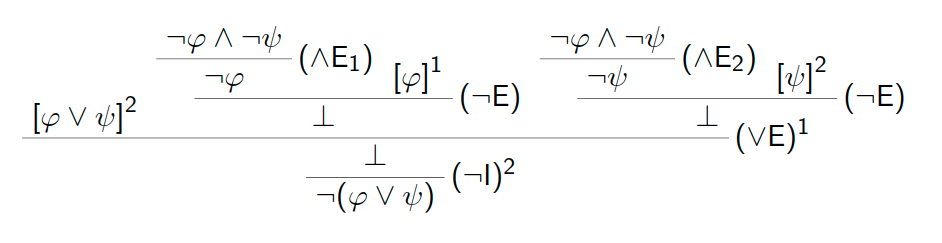
\includegraphics[width=\linewidth]{Assets/Logik-beispiel-1.png}

  \note{Satz}{Für jede Formel $\varphi$ ist $\lnot\lnot\varphi\rightarrow\varphi$ ein Theorem.}
  %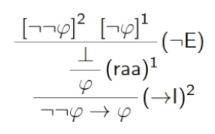
\includegraphics[width=\linewidth]{Assets/Logik-beispiel-5.png}

  \note{Satz}{Für jede Formel $\varphi$ ist $\varphi\vee\lnot\varphi$ ein Theorem.}
  %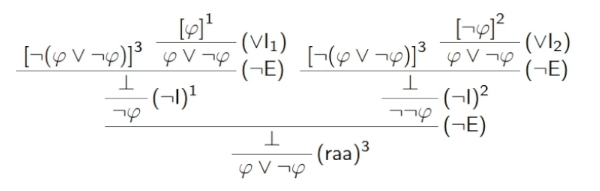
\includegraphics[width=\linewidth]{Assets/Logik-beispiel-6.png}

  \subsection{Semantik}
  Formeln sollen Verknüpfungen von Aussagen widerspiegeln.

  Idee der Semantik: wenn man jeder atomaren Formel $p_i$ einen Wahrheitswertzuordnet, so kann man den Wahrheitswert jeder Formel berechnen.

  Es gibt verschiedene Möglichkeiten, Wahrheitswerte zu definieren:
  \begin{itemize*}
    \item Boolesche Logik $B=\{0,1\}$: ''wahr''=1 und ''falsch''= 0
    \item dreiwertige Kleene-Logik $K_3=\{0,\frac{1}{2},1\}$: ''unbekannt''$=\frac{1}{2}$
    \item Fuzzy-Logik $F=[0,1]$: ''Grad der Überzeugtheit''
    \item unendliche Boolesche Algebra $B_R$= Menge der Teilmengen von $\mathbb{R}$
    \item Heyting-Algebra $H_R$= Menge der offenen Teilmengen von $\mathbb{R}$
  \end{itemize*}

  \subsection{Wahrheitswertebereiche}
  \note{Definition}{Sei W eine Menge und $R\subseteq W\times W$ eine binäre Relation.
    \begin{itemize*}
      \item R ist reflexiv, wenn $(a,a)\in R$ für alle $a\in W$ gilt.
      \item R ist antisymmetrisch, wenn $(a,b),(b,a)\in R$ impliziert, dass $a=b$ gilt (für alle $a,b\in W$).
      \item R ist transitive, wenn $(a,b),(b,c)\in R$ impliziert, dass $(a,c)\in R$ gilt (für alle $a,b,c\in W$).
      \item R ist eine Ordnungsrelation, wenn R reflexiv, antisymmetrisch und transitiv ist. In diesem Fall heißt das Paar $(W,R)$ eine partiell geordnete Menge.
    \end{itemize*}
  }

  \note{Definition}{Sei $(W,\leq)$ partiell geordnete Menge, $M\subseteq W$ und $a\in W$.
    \begin{itemize*}
      \item a ist obere Schranke von $M$, wenn $m\leq a$ für alle $m\in M$ gilt.
      \item a ist kleinste obere Schranke oder Supremum von $M$, wenn $a$ obere Schranke von $M$ ist und wenn $a\leq b$ für alle oberen Schranken $b$ von $M$ gilt. Wir schreiben in diesem Fall $a=sup \ M$.
      \item a ist untere Schranke von $M$, wenn $a\leq m$ für alle $m\in M$ gilt.
      \item a ist größte untere Schranke oder Infimum von $M$, wenn a untere Schranke von $M$ ist und wenn $b\leq a$ für alle unteren Schranken $b$ von $M$ gilt. Wir schreiben in diesem Fall $a=inf\ M$.
    \end{itemize*}
  }

  \note{Definition}{ Ein (vollständiger) Verband ist eine partiell geordnete Menge $(W,\leq)$, in der jede Menge $M\subseteq W$ ein Supremum $sup\ M$ und ein Infimum $inf\ M$ hat.}
  In einem Verband $(W,\leq)$ definieren wir:
  \begin{itemize*}
    \item $0_W = inf\ W$ und $1_W= sup\ W$
    \item $a\wedge_W b= inf\{a,b\}$ und $a\vee_W b= sup\{a,b\}$ für $a,b\in W$
  \end{itemize*}

  In jedem Verband $(W,\leq)$ gelten $0_W= sup\ \varnothing$ und $1_W= inf\ \varnothing$ (jedes Element von $W$ ist obere und untere Schranke von $\varnothing$).

  \note{Definition}{Ein Wahrheitswertebereich ist ein Tupel $(W,\leq,\rightarrow W,\lnot W)$, wobei $(W,\leq)$ ein Verband und $W\rightarrow W:W^2 \rightarrow W$ und $\lnot W:W\rightarrow W$  Funktionen sind.}

  \begin{itemize*}
    \item Boolesche Wahrheitswertebereich B mit Grundmenge $B=\{0,1\}$
    \begin{itemize*}
      \item $\lnot_B (a) = 1-a,\quad\rightarrow_B(a,b) = max(b, 1 -a)$
      \item $0_B=0,\quad 1_B= 1$,
      \item $a\wedge_B b= min(a,b),\quad a\vee_B b= max(a,b)$
    \end{itemize*}
    \item Kleenesche Wahrheitswertebereich $K_3=\{0,\frac{1}{2},1\}$
    \begin{itemize*}
      \item $\lnot_{K_3} (a) = 1 -a,\quad \rightarrow_{K_3} (a,b) = max(b, 1-a)$
      \item $\lnot_{K_3} = 0,\quad 1_{K_3} = 1$
      \item $a\wedge_{K_3} b= min(a,b),\quad a\vee_{K_3} b= max(a,b)$
    \end{itemize*}
    \item Fuzzy-Logik ist definiert durch Grundmenge $F=[0,1]\subseteq\mathbb{R}$
    \begin{itemize*}
      \item $\lnot_F (a) = 1-a,\quad\rightarrow_F (a,b) = max(b, 1-a)$
      \item $0_F= 0,\quad 1_F= 1$
      \item $a\wedge_F b= min(a,b),\quad a\vee_F b= max(a,b)$
    \end{itemize*}
    \item Boolesche Wahrheitswertebereich $B_R=\{A|A\subseteq \mathbb{R}\}$
    \begin{itemize*}
      \item $\lnot_{B_R} (A) =\mathbb{R}\backslash A,\quad \rightarrow_{B_R} (A,B) = B\cup\mathbb{R}\backslash A$
      \item $0_{B_R}=\varnothing,\quad 1_{B_R}=\mathbb{R}$
      \item $A\wedge_{B_R} B=A\cap B,\quad A\vee_{B_R} B=A\cup B$
    \end{itemize*}
    \item Heytingsche Wahrheitswertebereich $H_{\mathbb{R}} =\{A\subseteq\mathbb{R} | \text{A ist offen}\}$
    \begin{itemize*}
      \item $\lnot_{H_R} (A) = Inneres(\mathbb{R}\backslash A),\quad \rightarrow_{H_R} (A,B) =Inneres(B\cup \mathbb{R}\backslash A)$
      \item $0_{H_R}=\varnothing,\quad 1_{H_R}=\mathbb{R}$
      \item $A\wedge_{H_R} B= A\cap B,\quad A\vee_{H_R} B=A\cup B$
      \item $Inneres(A) =\{a\in A|\exists \epsilon > 0 : (a-\epsilon,a+\epsilon)\subseteq A\}$
    \end{itemize*}
  \end{itemize*}

  Sei W ein Wahrheitswertebereich und B eine W-Belegung. Induktiv über den Formelaufbau definieren wir den Wahrheitswert $\hat{B}(\phi)\in W$ jeder zu $B$ passenden Formel $\phi$:
  \begin{itemize*}
    \item $\hat{B}(\bot) = 0_W$
    \item $\hat{B}(p) = B(p)$ falls $p$ eine atomare Formel ist
    \item $\hat{B}((\phi\wedge \psi )) = \hat{B}(\phi)\wedge_W \hat{B}(\psi )$
    \item $\hat{B}((\phi\vee \psi )) = \hat{B}(\phi)\vee_W \hat{B}(\psi )$
    \item $\hat{B}((\phi\rightarrow \psi )) = \rightarrow W(\hat{B}(\phi),\hat{B}(\psi ))$
    \item $\hat{B}(\lnot\phi) = \lnot W(\hat{B}(\phi))$
  \end{itemize*}

  \subsection{Folgerung und Tautologie}
  Sei W ein Wahrheitswertebereich.
  Eine Formel $\phi$ heißt eine W-Folgerung der Formelmenge $\Gamma$, falls für jede W-Belegung B, die zu allen Formeln aus $\Gamma \cup\{\phi\}$ paßt, gilt: $inf\{B(\gamma )|\gamma \in \Gamma \}\leq B(\phi)$

  Wir schreiben $\Gamma \Vdash W\phi$, falls $\phi$ eine W-Folgerung von $\Gamma$ ist.

  Eine W-Tautologie ist eine Formel $\phi$ mit $\varnothing \Vdash W\phi$, d.h. $B(\phi) = 1_W$ für alle passenden W-Belegungen B.

  \subsection{Korrektheit}

  \note{Korrektheitslemma für nat. Schließen \& Wahrheitswertebereich B}{Sei $D$ eine Deduktion mit Hypothesen in der Menge $\Gamma$ und Konklusion $\varphi$. Dann gilt $\Gamma\vdash_B \varphi$, d.h. $inf\{B(\gamma)|\gamma\in\Gamma\}\leq B(\varphi)$ für alle passenden B-Belegungen $B$.}

  Beweis: Induktion über die Größe der Deduktion $D$ (d.h. Anzahl der Regelanwendungen).
  Ist die letzte Schlußregel in der Deduktion $D$ von der Form $(\wedge I), (\vee E), (\rightarrow I)$ oder $(raa)$, so ist die Behauptung des Lemmas gezeigt.

  \note{Korrektheitssatz für natürliches Schließen \& Wahrheitswertebereich $B$}{Für jede Menge von Formeln $\Gamma$ und jede Formel $\varphi$ gilt $\Gamma\vdash\varphi\Rightarrow\Gamma\vdash_B\varphi$.}

  Beweis: Wegen $\Gamma\vdash\varphi$ existiert eine Deduktion $D$ mit Hypothesen in $\Gamma$ und Konklusion $\varphi$. Nach dem Korrektheitslemma folgt $\Gamma\vdash_B \varphi$.

  \note{Korollar}{Jedes Theorem ist eine B-Tautologie.}
  \note{Korrektheitssatz für natürliches Schließen \& Wahrheitswertebereich $B$}{Für jede Menge von Formeln $\Gamma$ und jede Formel $\varphi$ gilt  $\Gamma\vdash\varphi\Rightarrow\Gamma\vdash_{B_\mathbb{R}}\varphi$.}

  Beweis: verallgemeinere den Beweis von Korrektheitslemma und Korrektheitssatz für $B$ auf $B_\mathbb{R}$ (Problem: wir haben mehrfach ausgenutzt, dass $B=\{0,1\}$ mit $0<1$)

  \note{Korollar}{Jedes Theorem ist eine $B_\mathbb{R}$-Tautologie.}

  \note{Korrektheitslemma für nat. Schließen \& Wahrheitswertebereich  $H_{\mathbb{R}}$ }{Sei $D$ eine Deduktion mit Hypothesen in der Menge $\Gamma$ und Konklusion $\varphi$, die die Regel $(raa)$ nicht verwendet. Dann gilt $\Gamma\vdash_{H_\mathbb{R}}\varphi$.}

  Beweis: ähnlich zum Beweis des Korrektheitslemmas für den Wahrheitswertebereich B. Nur die Behandlung der Regel $(raa)$ kann nicht übertragen werden.

  \note{Korrektheitssatz für nat. Schließen \& Wahrheitswertebereich $H_{\mathbb{R}}$ }{Für jede Menge von Formeln $\Gamma$ und jede Formel $\varphi$ gilt $\Gamma\vdash\varphi$ ohne $(raa)$ $\Rightarrow\Gamma\vdash_{H_{\mathbb{R}}}\varphi$.}

  \note{Korollar}{Jedes $(raa)$-frei herleitbare Theorem ist eine $H_{\mathbb{R}}$-Tautologie.}

  Folgerung: Jede Deduktion der Theoreme $\lnot\lnot\varphi\rightarrow\varphi$ und $\varphi\vee\lnot\varphi$ ohne Hypothesen verwendet $(raa)$.

  \subsection{Vollständigkeit}
  \begin{itemize*}
    \item Sei $W$ einer der Wahrheitswertebereiche $B,K_3 ,F ,B_\mathbb{R}, H_{\mathbb{R}}$
    \item z.z. ist $\Gamma\vdash_W\varphi\Rightarrow\Gamma\vdash\varphi$
    \item dies ist äquivalent zu $\Gamma\not\vdash\varphi\Rightarrow\Gamma\not\Vdash_W \varphi$
    \begin{itemize*}
      \item $\Gamma \not\Vdash_W\varphi$
      \item $\Leftrightarrow$ $\Gamma\cup\{\lnot\varphi\}$ konsistent
      \item $\Rightarrow$ $\exists\Delta\subseteq\Gamma\cup\{\lnot\varphi\}$ maximal konsistent
      \item $\Rightarrow$ $\Delta$ erfüllbar
      \item $\Rightarrow$ $\Gamma\cup\{\lnot\varphi\}$ erfüllbar
      \item $\Leftrightarrow$ $\Gamma\not\Vdash_B \varphi$
      \item $\Rightarrow$ $\Gamma\not\Vdash\varphi$
    \end{itemize*}
  \end{itemize*}

  \subsubsection{Konsistente Mengen}
  \note{Definition}{Sei $\Gamma$ eine Menge von Formeln. $\Gamma$ heißt inkonsistent, wenn $\Gamma\vdash\bot$ gilt. Sonst heißt $\Gamma$ konsistent.}

  \note{Lemma}{Sei $\Gamma$ eine Menge von Formeln und $\varphi$ eine Formel. Dann gilt $\Gamma\not\vdash\varphi \Leftrightarrow \Gamma\cup\{\lnot\varphi\}$ konsistent.}

  \subsubsection{Maximal konsistente Mengen}
  \note{Definition}{Eine Formelmenge $\Delta$ ist maximal konsistent, wenn sie konsistent ist und wenn gilt ''$\sum\supseteq\Delta$ konsistent $\Rightarrow\sum = \Delta$''.}

  \note{Satz}{Jede konsistente Formelmenge $\Gamma$ ist in einer maximal konsistenten Formelmenge $\Delta$ enthalten.}

  \note{Lemma 1}{Sei $\Delta$ maximal konsistent und gelte $\Delta\vdash\varphi$. Dann gilt $\varphi\in\Delta$.}

  \note{Lemma 2}{Sei $\Delta$ maximal konsistent und $\varphi$ Formel. Dann gilt $\varphi\not\in\Delta\Leftrightarrow\lnot\varphi\in\Delta$.}

  \subsection{Erfüllbare Mengen}
  \note{Definition}{Sei $\Gamma$ eine Menge von Formeln. $\Gamma$ heißt erfüllbar, wenn es eine passende B-Belegung $B$ gibt mit $B(\gamma) = 1_B$ für alle $\gamma\in\Gamma$.}
  \begin{itemize*}
    \item Die Erfüllbarkeit einer endlichen Menge $\Gamma$ ist entscheidbar:
    \item Berechne Menge $V$ von in $\Gamma$ vorkommenden atomaren Formeln
    \item Probiere alle B-Belegungen $B:V\rightarrow B$ durch
    \item Die Erfüllbarkeit einer endlichen Menge $\Gamma$ ist NP-vollständig (Satz von Cook)
  \end{itemize*}

  \note{Satz}{Sei $\Delta$  eine maximal konsistente Menge von Formeln. Dann ist $\Delta$ erfüllbar.}

  Beweis: Definiere eine B-Belegung $B$ mittels $B(p_i) = \begin{cases} 1_B \quad\text{ falls } p_i\in\Delta \\ 0_B \quad\text{ sonst. } \end{cases}$
  Wir zeigen für alle Formeln $\varphi: B(\varphi) = 1_B \Leftarrow\Rightarrow\varphi\in\Delta$ (*)

  Der Beweis erfolgt per Induktion über die Länge von $\varphi$

  \note{Lemma}{Sei $\Gamma$ eine Menge von Formeln und $\varphi$ eine Formel. Dann gilt $\Gamma\not\Vdash_B\varphi\Leftarrow\Rightarrow\Gamma\cup\{\lnot \varphi\}$ erfüllbar.}

  \note{Beobachtung}{Sei $W$ einer der Wahrheitswertebereiche $B, K_3, F, H_R$ und $B_R,\Gamma$ eine Menge von Formeln und $\varphi$ eine Formel. Dann gilt $\Gamma\Vdash W\varphi\Rightarrow\Gamma\Vdash B\varphi$.}

  \note{Satz (Vollständigkeitssatz)}{Sei $\Gamma$ eine Menge von Formeln, $\varphi$ eine Formel und $W$ einer der Wahrheitswertebereiche $B,K_3 , F, B_R$ und $H_R$. Dann gilt $\Gamma\Vdash_W\varphi \Rightarrow \Gamma\vdash\varphi$. Insbesondere ist jede W-Tautologie ein Theorem.}

  Beweis (indirekt)
  \begin{itemize*}
    \item $\Gamma\not\Vdash$
    \item $\Gamma\cup\{\lnot\varphi\}$ konsistent
    \item $\exists\Delta\supseteq\Gamma\cup\{\lnot\varphi\}$ maximal konsistent
    \item $\Rightarrow\Delta$ erfüllbar
    \item $\Gamma\cup\{\lnot\varphi\}$ erfüllbar
    \item $\Gamma\not\Vdash_B \varphi$
    \item $\Gamma\not\Vdash_W \varphi$
  \end{itemize*}

  \subsection{Vollständigkeit und Korrektheit}
  \note{Satz}{Seien $\Gamma$ eine Menge von Formeln und $\varphi$ eine Formel. Dann gilt $\Gamma\vdash\varphi\Leftarrow\Rightarrow\Gamma\Vdash_B \varphi$. Insbesondere ist eine Formel genau dann eine B-Tautologie, wenn sie ein Theorem ist.}

  Beweis: Folgt unmittelbar aus Korrektheitssatz und Vollständigkeitssatz.

  Bemerkung:
  \begin{itemize*}
    \item gilt für jede ''Boolesche Algebra'', z.B. $B_R$
    \item $\Gamma\vdash\varphi$ ohne ($raa$) $\Leftarrow\Rightarrow\Gamma\Vdash_{H_R} \varphi$ (Tarksi 1938)
  \end{itemize*}


  \subsubsection{Folgerung 1: Entscheidbarkeit}
  \note{Satz}{die Menge der Theoreme ist entscheidbar.}

  Beweis: Sei $\varphi$ Formel und $V$ die Menge der vorkommenden atomaren Formeln. Dann gilt $\varphi$ Theorem
  \begin{itemize*}
    \item $\Leftarrow\Rightarrow\varphi$ B-Tautologie
    \item $\Leftarrow\Rightarrow$ für alle Abbildungen $B:V\rightarrow\{0_B, 1_B\}$ gilt $B(\varphi) = 1_B$
  \end{itemize*}

  Da es nur endlich viele solche Abbildungen gibt und $B(\varphi)$ berechnet werden kann, ist dies eine entscheidbare Aussage.

  \subsubsection{Folgerung 2: Äquivalenzen und Theoreme}
  \note{Definition}{Zwei Formeln $\alpha$ und $\beta$ heißen äquivalent $(\alpha\equiv\beta)$, wenn für alle passenden B-Belegungen $B$ gilt: $B(\alpha) =B(\beta)$.}

  Es gelten die folgenden Äquivalenzen:
  \begin{enumerate*}
    \item $p_1 \vee p_2 \equiv p_2 \vee p_1$
    \item $(p_1 \vee p_2 )\vee p_3 \equiv p_1 \vee (p_2 \vee p_3 )$
    \item $p_1 \vee (p_2 \wedge p_3 )\equiv (p_1 \vee p_2 )\wedge (p_1 \vee p_3 )$
    \item $\lnot(p_1 \vee p_2 )\equiv\lnot p_1 \wedge\lnot p_2$
    \item $p_1 \vee p_1 \equiv p_1$
    \item $(p_1 \wedge \lnot p_1 )\vee p_2 \equiv p_2$
    \item $\lnot\lnot p_1\equiv p_1$
    \item $p_1 \wedge\lnot p_1 \equiv\bot$
    \item $p_1 \vee\lnot p_1 \equiv\lnot\bot$
    \item $p_1 \rightarrow p_2 \equiv \lnot p_1 \vee p_2$
  \end{enumerate*}

  Bemerkung: Mit den üblichen Rechenregeln für Gleichungen können aus dieser Liste alle gültigen Äquivalenzen hergeleitet werden.

  \paragraph{Zusammenhang zw. Theoremen und Äquivalenzen}
  \note{Satz}{Seien $\alpha$ und $\beta$ zwei Formeln. Dann gilt $\alpha\equiv\beta\Leftarrow\Rightarrow(\alpha\leftrightarrow\beta)$ ist Theorem.}

  \note{Satz}{Sei $\alpha$ eine Formel. Dann gilt $\alpha$ ist Theorem $\Leftarrow\Rightarrow\alpha\equiv\lnot\bot$.}

  \subsubsection{Folgerung 3: Kompaktheit}
  \note{Satz}{Sei $\Gamma$ eine u.U. unendliche Menge von Formeln und $\varphi$ eine Formel mit $\Gamma\Vdash_B\varphi$. Dann existiert $\Gamma'\subseteq\Gamma$ endlich mit $\Gamma'\Vdash_B \varphi$.}

  \note{Folgerung (Kompaktheits- oder Endlichkeitssatz)}{Sei $\Gamma$ eine u.U. unendliche Menge von Formeln. Dann gilt $\Gamma$ unerfüllbar $\Leftarrow\Rightarrow\exists\Gamma'\subseteq\Gamma$ endlich: $\Gamma'$ unerfüllbar}

  \subsubsection{1. Anwendung des Kompaktheitsatzes: Färbbarkeit}
  \note{Definition}{Ein Graph ist ein Paar $G=(V,E)$ mit einer Menge $V$ und $E\subseteq\binom{V}{2} =\{X\subseteq V:|V\Vdash 2\}$. Für $W\subseteq V$ sei $G\upharpoonright_W= (W,E\cap\binom{W}{2})$ der von $W$ induzierte Teilgraph. Der Graph G ist 3-färbbar, wenn es eine Abbildung $f:V\rightarrow\{1,2,3\}$ mit $f(v)\not=f(w)$ für alle $\{v,w\}\in E$.}

  Bemerkung: Die 3-Färbbarkeit eines endlichen Graphen ist NP-vollständig

  \note{Satz}{Sei $G= (N,E)$ ein Graph. Dann sind äquivalent
    \begin{enumerate*}
      \item $G$ ist 3-färbbar.
      \item Für jede endliche Menge $W\subseteq N$ ist $G\upharpoonright_W$ 3-färbbar.
    \end{enumerate*}
  }

  Behauptung: Jede endliche Menge $\Delta\subseteq\Gamma$ ist erfüllbar.

  Nach dem Kompaktheitssatz ist $\Gamma$ erfüllbar.
  Sei $B$ erfüllende Belegung. Für $n\in N$ existiert genau ein $c\in\{1,2,3\}$ mit $B(p_{n,c}) =1$. Setze $f(n) =c$. Dann ist $f$ eine gültige Färbung des Graphen $G$.

  \subsubsection{2. Anwendung des Kompaktheitsatzes: Parkettierungen}

  \note{Definition}{Ein Kachelsystem besteht aus einer endlichen Menge C von ''Farben'' und einer Menge K von Abbildungen $\{N,O,S,W\}\rightarrow C$ von ''Kacheln''.
    Eine Kachelung von $G\subseteq Z\times Z$ ist eine Abbildung $f:G\rightarrow K$ mit
    \begin{itemize*}
      \item $f(i,j)(N) =f(i,j+ 1 )(S)$ für alle $(i,j),(i,j+ 1 )\in G$
      \item $f(i,j)(O) =f(i+ 1 ,j)(W)$ für alle $(i,j),(i+ 1 ,j)\in G$
    \end{itemize*}
  }

  \note{Satz}{Sei $K$ ein Kachelsystem. Es existiert genau dann eine Kachelung von $Z\times Z$, wenn für jedes $n\in N$ eine Kachelung von $\{(i,j) :|i|,|j| \leq n\}$ existiert.}

  Bemerkung: Der Kompaktheitssatz gilt auch, wenn die Menge der atomaren Formeln nicht abzählbar ist.

  \subsection{Erfüllbarkeit}
  \note{Erfüllbarkeitsproblem}{
    Eingabe: Formel $\Gamma$.

    Frage: existiert eine B-Belegung $B$ mit $B(\Gamma) = 1_B$.}

  \subsubsection{Hornformeln (Alfred Horn, 1918-2001)}
  \note{Definition}{Eine Hornklausel hat die Form $(\lnot\bot\wedge p_1\wedge p_2\wedge ... \wedge p_n)\rightarrow q$ für $n\geq 0$, atomare Formeln $p_1 ,p_2 ,... ,p_n$ und $q$ atomare Formel oder $q=\bot$.
    Eine Hornformel ist eine Konjunktion von Hornklauseln.}

  \begin{itemize*}
    \item $\{p_1,p_2 ,... ,p_n\}\rightarrow q$ für Hornklausel $(\lnot\bot\wedge p_1 \wedge p_2 \wedge ...\wedge p_n)\rightarrow q$
    insbes. $\varnothing\rightarrow q$ für $\lnot\bot\rightarrow q$
    \item $\{(M_i\rightarrow q_i)| 1 \leq i\leq n\}$ für Hornformel $\bigwedge_{1 \leq i \leq n} (M_i\rightarrow q_i)$
  \end{itemize*}

  Bemerkung, in der Literatur auch:
  \begin{itemize*}
    \item $\{\lnot p_1,\lnot p_2 ,... ,\lnot p_n,q\}$ für $\{p_1 ,... ,p_n\}\rightarrow q$ mit $q$ atomare Formel
    \item $\{\lnot p_1,\lnot p_2 ,... ,\lnot p_n\}$ für $\{p_1 ,... ,p_n\}\rightarrow\bot$
    \item $\Box$ für $\varnothing\rightarrow\bot$, die ''leere Hornklausel''
  \end{itemize*}

  \subsubsection{Markierungsalgorithmus}
  Eingabe: eine endliche Menge $\Gamma$ von Hornklauseln.
  \begin{enumerate*}
    \item while es gibt in $\Gamma$ eine Hornklausel $M\rightarrow q$, so dass alle $p\in M$ markiert sind und $q$ unmarkierte atomare Formel ist:
    do markiere $q$ (in allen Hornklauseln in $\Gamma$)
    \item if $\Gamma$ enthält eine Hornklausel der Form $M\rightarrow\bot$, in der alle $p\in M$ markiert sind
    then return ''unerfüllbar''
    else return ''erfüllbar''
  \end{enumerate*}

  \begin{enumerate*}
    \item Der Algorithmus terminiert: in jedem Durchlauf der while-Schleife wird wenigstens eine atomare Formel markiert. Nach endlich vielen Schritten terminiert die Schleife also.
    \item Wenn der Algorithmus eine atomare Formel q markiert und wenn $B$ eine B-Belegung ist, die $\Gamma$ erfüllt, dann gilt $B(q) = 1_B$.
    Beweis: wir zeigen induktiv über $n$: Wenn $q$ in einem der ersten $n$ Schleifendurchläufe markiert wird, dann gilt $B(q) = 1_B$.
    \item Wenn der Algorithmus ''unerfüllbar'' ausgibt, dann ist $\Gamma$ unerfüllbar.
    Beweis: indirekt, wir nehmen also an, dass der Algorithmus ''unerfüllbar'' ausgibt, $B$ aber eine B-Belegung ist, die $\Gamma$ erfüllt.
    \item Wenn der Algorithmus ''erfüllbar'' ausgibt, dann erfüllt die folgende B-Belegung alle Formeln aus $\Gamma$:
    $B(p_i)=\begin{cases} 1_B \quad\text{ der Algorithmus markiert } p_i \\ 0_B \quad\text{ sonst} \end{cases}$
    \item Also gilt $B(M\rightarrow q) = 1_B$ für alle Hornklauseln aus $\Gamma$, d.h. $\Gamma$ ist erfüllbar.
  \end{enumerate*}

  \note{Satz}{Sei $\Gamma$ endliche Menge von Hornklauseln. Dann terminiert der Markierungsalgorithmus mit dem korrekten Ergebnis.}

  Beweis: Die Aussagen 1.-4. beweisen diesen Satz.

  Bemerkungen:
  \begin{itemize*}
    \item Mit einer geeigneten Implementierung läuft der Algorithmusin linearer Zeit.
    \item Wir haben sogar gezeigt, dass bei Ausgabe von ''erfüllbar'' eine erfüllende B-Belegung berechnet werden kann.
  \end{itemize*}

  \subsubsection{SLD-Resolution}
  \note{Definition}{Sei $\Gamma$ eine Menge von Hornklauseln. Eine SLD-Resolution aus $\Gamma$ ist eine Folge $(M_0\rightarrow\bot,M_1\rightarrow\bot,... ,M_m\rightarrow\bot)$ von Hornklauseln mit
    \begin{itemize*}
      \item $(M_0\rightarrow\bot)\in\Gamma$
      \item für alle $0\leq n<m$ existiert $(N\rightarrow q)\in\Gamma$ mit $q\in M_n$ und $M_{n+1} = M_n\backslash\{q\}\cup N$
    \end{itemize*}
  }

  Beispiel:
  \begin{itemize*}
    \item $\Gamma =\{\{BH\}\rightarrow AK,\{AK,BH\}\rightarrow\bot,\{RL,AK\}\rightarrow BH,\varnothing\rightarrow RL,\varnothing\rightarrow AK\}$
    \item $M_0 =\{AK,BH\}$
    \item $M_1 =M_0 \backslash\{BH\}\cup\{RL,AK\}=\{RL,AK\}$
    \item $M_2 =M_1 \backslash\{RL\}\cup\varnothing =\{AK\}$
    \item $M_3 =M_2 \backslash\{AK\}\cup\varnothing =\varnothing$
  \end{itemize*}

  \note{Lemma A}{Sei $\Gamma$ eine (u.U. unendliche) Menge von Hornklauseln und $(M_0\rightarrow\bot, M_1\rightarrow\bot,... , M_m\rightarrow\bot)$ eine SLD-Resolution aus $\Gamma$ mit $M_m=\varnothing$. Dann ist $\Gamma$ nicht erfüllbar.}

  \note{Lemma B}{Sei $\Gamma$ eine (u.U. unendliche) unerfüllbare Menge von Hornklauseln. Dann existiert eine SLD-Resolution $(M_0\rightarrow\bot,...,M_m\rightarrow\bot)$ aus $\Gamma$ mit $M_m=\varnothing$.}

  Beweis: Endlichkeitssatz: es gibt $\Delta\subseteq\Gamma$ endlich und unerfüllbar. Bei Eingabe von$\Delta$ terminiert Markierungsalgorithmus mit ''unerfüllbar''
  \begin{itemize*}
    \item $r\geq 0...$ Anzahl der Runden
    \item $q_i...$ Atomformel, die in $i$ Runde markiert wird $(1\leq i\leq r)$
  \end{itemize*}

  Behauptung: Es gibt $m\leq r$ und SLD-Resolution $(M_0\rightarrow\bot,...,M_m\rightarrow\bot)$ aus $\Delta$ mit $M_m=\varnothing$ und $M_n\subseteq\{q_1,q_2,... ,q_{r-n}\}$ f.a. $0\leq n\leq m$. (5)

  \note{Satz}{Sei $\Gamma$ eine (u.U. unendliche) Menge von Hornklauseln. Dann sind äquivalent:
    \begin{enumerate*}
      \item $\Gamma$ ist nicht erfüllbar.
      \item Es gibt eine SLD-Resolution $(M_0\rightarrow\bot,M_1\rightarrow\bot,... ,M_m\rightarrow\bot)$ aus $\Gamma$ mit $M_m=\varnothing$.
    \end{enumerate*}
  }

  Die Suche nach einer SLD-Resolution mit $M_m=\varnothing$ kann grundsätzlich auf zwei Arten erfolgen:
  \begin{itemize*}
    \item Breitensuche:
    \begin{itemize*}
      \item findet SLD-Resolution mit $M_m=\varnothing$ (falls sie existiert), da Baum endlich verzweigend ist (d.h. Niveaus sind endlich)
      \item hoher Platzbedarf, da ganze Niveaus abgespeichert werden müssen (in einem Binärbaum der Tiefe $n$ kann es Niveaus der Größe $2^n$ geben)
    \end{itemize*}
    \item Tiefensuche:
    \begin{itemize*}
      \item geringerer Platzbedarf (in einem Binärbaum der Tiefe $n$ hat jeder Ast die Länge $\leq n$)
      \item findet existierende SLD-Resolution mit $M_m=\varnothing$ nicht immer
    \end{itemize*}
  \end{itemize*}

  \section{Kapitel 2: Prädikatenlogik}
  Um über Graphen Aussagen in der Aussagenlogik zu machen, verwenden wir Formeln $\varphi_{i,j}$ für $1\leq i,j\leq 9$ mit $\varphi_{i,j}=\begin{cases} \lnot\bot\quad\text{ falls} (v_i,v_j) Kante\\ \bot\quad\text{ sonst}\end{cases}$
  \begin{itemize*}
    \item Die aussagenlogische Formel $\bigvee_{1\leq i,j\leq 9} \varphi_{i,j}$ sagt aus, dass der Graph eine Kante enthält.
    \item Die aussagenlogische Formel $\bigwedge_{1\leq i\leq 9} \bigvee_{1\leq j\leq 9} \varphi_{i,j}$ sagt aus, dass jeder Knoten einen Nachbarn hat
    \item Die aussagenlogische Formel $\bigvee_{1\leq i,j,k\leq 9 verschieden} \varphi_{i,j}\wedge\varphi_{j,k}\wedge\varphi_{k,i}$ sagt aus, dass der Graph ein Dreieck enthält.
  \end{itemize*}

  \subsection{Kodierung in einer Struktur}
  \begin{itemize*}
    \item Grundmenge
    \item Teilmengen
    \item Relationen: Enthaltensein in einer Teilmenge oder Beziehungen zwischen Objekten ausdrücken
    \item Funktion: Objekte auf andere Objekte abbilden
    \item Konstante: Nullstellige Funktionen (ohne Argumente)
  \end{itemize*}

  \subsection{Syntax der Prädikatenlogik}

  \note{Definition}{Eine Signatur ist ein Tripel $\sum=(\Omega, Rel,ar)$, wobei $\Omega$ und $Rel$ disjunkte Mengen von Funktions- und Relationsnamen sind und $ar:\Omega\cup Rel\rightarrow\mathbb{N}$ eine Abbildung ist.}

  Beispiel: $\Omega=\{f,dk\}$ mit $ar(f) =1,ar(dk)=0$

  \note{Definition}{Die Menge der Variablen ist $Var=\{x_0,x_1 ,...\}$.}

  \note{Definition}{Sei $\sum$ eine Signatur. Die Menge $T_{\sum}$ der $\sum$-Terme ist induktiv definiert:
    \begin{enumerate*}
      \item Jede Variable ist ein Term, d.h. $Var\subseteq T_{\sum}$
      \item ist $f\in\Omega$ mit $ar(f)=k$ und sind $t_1,...,t_k\in T_{\sum}$, so gilt $f(t_1,...,t_k)\in T_{\sum}$
      \item Nichts ist $\sum$-Term, was sich nicht mittels der obigen Regeln erzeugen läßt.
    \end{enumerate*}
  }

  \note{Definition}{Sei $\sum$ Signatur. Die atomaren $\sum$-Formeln sind die Zeichenketten der Form
    \begin{itemize*}
      \item $R(t_1,t_2,...,t_k)$ falls $t_1,t_2,...,t_k\in T_{\sum}$ und $R\in Rel$ mit $ar(R)=k$ oder
      \item $t_1=t_2$ falls $t_1,t_2\in T_{\sum}$ oder
      \item $\bot$.
    \end{itemize*}
  }

  \note{Definition}{Sei $\sum$ Signatur. $\sum$-Formeln werden durch folgenden induktiven Prozeß definiert:
    \begin{enumerate*}
      \item Alle atomaren $\sum$-Formeln sind $\sum$-Formeln.
      \item Falls $\varphi$ und $\Psi$ $\sum$-Formeln sind, sind auch $(\varphi\wedge\Psi)$,$(\varphi\vee\Psi)$ und $(\varphi\rightarrow\Psi)$ $\sum$-Formeln.
      \item Falls $\varphi$ eine $\sum$-Formel ist, ist auch $\lnot\varphi$ eine $\sum$-Formel.
      \item Falls $\varphi$ eine $\sum$-Formel und $x\in Var$, so sind auch $\forall x\varphi$ und $\exists x\varphi$ $\sum$-Formeln.
      \item Nichts ist $\sum$-Formel, was sich nicht mittels der obigen Regeln erzeugen läßt.
    \end{enumerate*}
  }

  \note{Definition}{Sei $\sum$ eine Signatur. Die Menge $FV(\varphi)$ der freien Variablen einer $\sum$-Formel $\varphi$ ist induktiv definiert:
    \begin{itemize*}
      \item Ist $\varphi$ atomare $\sum$-Formel, so ist $FV(\varphi)$ die Menge der in $\varphi$ vorkommenden Variablen.
      \item $FV(\varphi\Box\Psi) =FV(\varphi)\cup FV(\Psi)$ für $\Box\in\{\wedge,\vee,\rightarrow\}$
      \item $FV(\lnot\varphi) =FV(\varphi)$
      \item $FV(\exists x\varphi) =FV(\forall x\varphi) =FV(\varphi)\backslash\{x\}$.
    \end{itemize*}
    Eine $\sum$-Formel $\varphi$ ist geschlossen oder ein $\sum$-Satz, wenn $FV(\varphi)=\varnothing$ gilt.}

  \note{Definition}{Sei $\sum$ eine Signatur. Eine $\sum$-Struktur ist ein Tupel $A=(U_A,(f^A)_{f\in\Omega},(R^A)_{R\in Rel})$, wobei
    \begin{itemize*}
      \item $U_A$ eine nichtleere Menge, das Universum,
      \item $R^A\supseteq U_A^{ar(R)}$ eine Relation der Stelligkeit $ar(R)$ für $R\in Rel$ und
      \item $f^A:U_A^{ar(f)}\rightarrow U_A$ eine Funktion der Stelligkeit $ar(f)$ für $f\in\Omega$ ist.
    \end{itemize*}
  }

  Bemerkung: $U_A^0=\{()\}$.
  \begin{itemize*}
    \item Also ist $a^A:U_A^0\rightarrow U_A$ für $a\in\Omega$ mit $ar(a)=0$ vollständig gegeben durch $a^A(())\in U_A$. Wir behandeln 0-stellige Funktionen daher als Konstanten.
    \item Weiterhin gilt $R^A=\varnothing$ oder $R^A=\{()\}$ für $R\in Rel$ mit $ar(R)=0$.
  \end{itemize*}

  \note{Definition}{Sei $\sum$ eine Signatur, $\varphi$ eine $\sum$-Formel, $\Delta$ eine Menge von $\sum$-Formeln und $A$ eine $\sum$-Struktur.
    \begin{itemize*}
      \item $A\Vdash\varphi$ ($A$ ist Modell von $\varphi$) falls $A\Vdash_p\varphi$ für alle Variableninterpretationen $\rho$ gilt.
      \item $A\Vdash\Delta$ falls $A\Vdash\Psi$ für alle $\Psi\in\Delta$.
    \end{itemize*}
  }

  \note{Definition}{Sei $\sum$ eine Signatur, $\varphi$ eine $\sum$-Formel, $\Delta$ eine Menge von $\sum$-Formeln und $A$ eine $\sum$-Struktur.
    \begin{itemize*}
      \item $\Delta$ ist erfüllbar, wenn es $\sum$-Struktur $B$ und Variableninterpretation $\rho:Var\rightarrow U_B$ gibt mit $B\Vdash_\rho\Psi$ für alle $\Psi\in\Delta$.
      \item $\varphi$ ist semantische Folgerung von $\Delta(\Delta\Vdash\varphi)$ falls für alle $\sum$-Strukturen $B$ und alle Variableninterpretationen $\rho:Var\rightarrow U_B$ gilt: Gilt $B\Vdash_\rho\Psi$ für alle $\Psi\in\Delta$, so gilt auch $B\Vdash_\rho \varphi$.
      \item $\varphi$ ist allgemeingültig, falls $B\Vdash \rho\varphi$ für alle $\sum$-Strukturen $B$ und alle Variableninterpretationen $\rho$ gilt.
    \end{itemize*}
  }

  Bemerkung: $\varphi$ allgemeingültig gdw. $\varnothing\Vdash\varphi$ gdw. $\{\lnot\varphi\}$ nicht erfüllbar. Hierfür schreiben wir auch $\Vdash\varphi$.

  \subsection{Substitutionen}
  \note{Definition}{Eine Substitution besteht aus einer Variable $x\in Var$ und einem Term $t\in T_{\sum}$, geschrieben $[x:=t]$.}

  Die Formel $\varphi[x:=t]$ ist die Anwendung der Substitution $[x:=t]$ auf die Formel $\varphi$. Sie entsteht aus $\varphi$, indem alle freien Vorkommen von $x$ durch $t$ ersetzt werden. Sie soll das über $t$ aussagen, was $\varphi$ über $x$ ausgesagt hat.

  \note{Lemma}{Seien $\sum$ Signatur, $A$ $\sum$-Struktur, $\rho:Var\rightarrow U_A$ Variableninterpretation, $x\in Var$ und $s,t\in T_{\sum}$. Dann gilt $\rho(s[x:=t])=\rho[x\rightarrow \rho(t)](s)$.}

  \note{Definition}{Sei $[x:=t]$ Substitution und $\varphi$ $\sum$-Formel. Die Substitution $[x:=t]$ heißt für $\varphi$ zulässig, wenn für alle $y\in Var$ gilt: $y$ Variable in $t\Rightarrow\varphi$ enthält weder $\exists y$ noch $\forall y$}

  \note{Lemma}{Sei $\sum$ Signatur, A $\sum$-Struktur, $\rho:Var\rightarrow U_A$ Variableninterpretation, $x\in Var$ und $t\in T_{\sum}$. Ist die Substitution $[x:=t]$ für die $\sum$-Formel $\varphi$ zulässig, so gilt $A\Vdash_p\varphi [x:=t]\Leftrightarrow  A\Vdash_{p[x\rightarrow \rho(t)]}\varphi$.}

  \subsection{Korrektheit}
  Der Beweis des Korrektheitslemmas für das natürliche Schließen kann ohne große Schwierigkeiten erweitert werden.

  \note{Lemma V0}{Sei $\sum$ eine Signatur, $\Gamma$ eine Menge von $\sum$-Formeln und $\varphi$ eine $\sum$-Formel. Sei weiter $D$ eine Deduktion mit Hypothesen in $\Gamma$ und Konklusion $\varphi$, die die Regeln des natürlichen Schließens der Aussagenlogik verwendet. Dann gilt $\Gamma\Vdash\varphi$.}

  Umgekehrt ist nicht zu erwarten, dass aus $\Gamma\Vdash\varphi$ folgt, dass es eine Deduktion mit Hypothesen in $\Gamma$ und Konklusion $\varphi$ gibt, denn die bisher untersuchten Regeln erlauben keine Behandlung von $=,\forall$ bzw. $\exists$. Solche Regeln werden wir jetzt einführen.

  Zunächst kümmern wir uns um Atomformeln der Form $t_1 =t_2$. Hierfür gibt es die zwei Regeln $(R)$ und $(GfG)$:

  \note{Reflexivität}{Für jeden Term $t$ ist $\frac{}{t=t}$ eine hypothesenlose Deduktion mit Konklusion $t=t$.  %\includegraphics[width=\linewidth]{Assets/Logik-reflexivität-kurz.png}
  }

  \note{Gleiches-für-Gleiches}{Seien $s$ und $t$ Terme und $\varphi$ Formel, so dass die Substitutionen $[x:=s]$ und $[x:=t]$ für $\varphi$ zulässig sind. Sind $D$ und $E$ Deduktionen mit Hypothesen in $\Gamma$ und Konklusionen $\varphi[x:=s]$ bzw. $s=t$, so ist das folgende eine Deduktion mit Hypothesen in $\Gamma$ und Konklusion $\varphi[x:=t]$
    %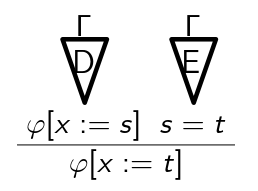
\includegraphics[width=\linewidth]{Assets/Logik-gleiches-für-gleiches-ausführlich.png)
  }

  Bedingung: über keine Variable aus $s$ oder $t$ wird in $\varphi$ quantifiziert

  \note{Lemma V1}{Sei $\sum$ eine Signatur, $\Gamma$ eine Menge von $\sum$-Formeln und $\varphi$ eine $\sum$-Formel. Sei weiter $D$ eine Deduktion mit Hypothesen in $\Gamma$ und Konklusion $\varphi$, die die Regeln des natürlichen Schließens der Aussagenlogik, $(R)$ und $(GfG)$ verwendet. Dann gilt $\Gamma\Vdash\varphi$.}

  \note{$\forall$-Einführung}{ Sei $D$ eine Deduktion mit Hypothesen in $\Gamma$ und Konklusion $\varphi$ und sei $x$ eine Variable, die in keiner Formel aus $\Gamma$ frei vorkommt. Dann ist das folgende eine Deduktion mit Hypothesen in $\Gamma$ und Konklusion $\forall x\varphi: \frac{\phi}{\forall x\varphi}$

    Bedingung: $x$ kommt in keiner Hypothese frei vor}

  \note{Lemma V2}{Sei $\sum$ eine Signatur, $\Gamma$ eine Menge von $\sum$-Formeln und $\varphi$ eine $\sum$-Formel. Sei weiter $D$ eine Deduktion mit Hypothesen in $\Gamma$ und Konklusion $\varphi$, die die Regeln des natürlichen Schließens der Aussagenlogik, (R), (GfG) und ($\forall$ -I) verwendet. Dann gilt $\Gamma\Vdash\varphi$.}

  \note{$\forall$ -Elimination}{Sei $D$ eine Deduktion mit Hypothesen in $\Gamma$ und Konklusion $\forall x\varphi$ und seit Term, so dass Substitution [x:=t] für $\varphi$ zulässig ist. Dann ist das folgende eine Deduktion mit Hypothesen in $\Gamma$ und Konklusion $\varphi[x:=t]:\frac{\forall x\varphi}{\varphi[x:=t]}$

    Bedingung: über keine Variable aus $t$ wird in $\varphi$ quantifiziert}

  \note{Lemma V3}{ Sei $\sum$ eine Signatur, $\Gamma$ eine Menge von $\sum$-Formeln und $\varphi$ eine $\sum$-Formel. Sei weiter $D$ eine Deduktion mit Hypothesen in $\Gamma$ und Konklusion $\varphi$, die die Regeln des natürlichen Schließens der Aussagenlogik, (R), (GfG), ($\forall$-I) und ($\forall$-E) verwendet. > Dann gilt $\Gamma\Vdash\varphi$.}

  \note{$\exists$ -Elimination}{Sei $\Gamma$ eine Menge von Formeln, die die Variable $x$ nicht frei enthalten und enthalte die Formel $\sigma$  die Variabel $x$ nicht frei. Wenn $D$ eine Deduktion mit Hypothesen in $\Gamma$ und Konklusion $\exists x\varphi$ und $E$ eine Deduktion mit Hypothesen in $\Gamma\cup\{\varphi\}$ und Konklusion $\sigma$ ist, dann ist das folgende eine Deduktion mit Hypothesen in $\Gamma$ und Konklusion $\sigma:\frac{\exists x\varphi \quad\quad \sigma}{\sigma}$

    Bedingung: $x$ kommt in den Hypothesen und in $\sigma$ nicht frei vor.}

  \note{Lemma V4}{Sei $\sigma$ eine Signatur, $\Gamma$ eine Menge von $\sum$-Formeln und $\varphi$ eine $\sigma$ -Formel. Sei weiter $D$ eine Deduktion mit Hypothesen in $\Gamma$ und Konklusion $\varphi$, die die Regeln des natürlichen Schließens der Aussagenlogik, (R), (GfG), ($\forall$-I), ($\forall$-E) und ($\exists$-E) verwendet. Dann gilt $\Gamma\Vdash\varphi$.}

  \note{$\exists$ -Einführung}{Sei die Substitution $[x:=t]$ für die Formel $\varphi$ zulässig. Sei weiter $D$ eine Deduktion mit Hypothesen in $\Gamma$ und Konklusion $\varphi[x:=t]$. Dann ist das folgende eine Deduktion mit Hypothesen in $\Gamma$ und Konklusion $\exists x\varphi:\frac{\varphi[x:=t]}{\exists x\varphi}$

    Bedingung: über keine Variable in $t$ wird in $\varphi$ quantifiziert}

  \note{Korrektheitslemma für das natürliche Schließen in der Prädikatenlogik}{
    Sei $\sigma$ eine Signatur, $\Gamma$ eine Menge von $\sum$-Formeln und $\varphi$ eine $\sigma$ -Formel.
    Sei weiter $D$ eine Deduktion mit Hypothesen in $\Gamma$ und Konklusion $\varphi$, die die Regeln des natürlichen Schließens der Aussagenlogik, (R), (GfG), ($\forall$-I), ($\forall$-E), ($\exists$ -E) und ($\exists$ -I) verwendet. Dann gilt $\Gamma\Vdash\varphi$.}

  \note{Definition}{Für eine Menge $\Gamma$ von $\sum$-Formeln und eine $\sum$-Formel $\varphi$ schreiben wir $\Gamma\vdash\varphi$ wenn es eine Deduktion gibt mit Hypothesen in $\Gamma$ und Konklusion $\varphi$. Wir sagen ''$\varphi$ ist eine syntaktische Folgerung von $\Gamma$''.
    Eine Formel $\varphi$ ist ein Theorem, wenn $\varnothing\vdash\varphi$ gilt.}

  \note{Korrektheitssatz}{Für eine Menge von $\sum$-Formeln $\Gamma$ und eine $\sum$-Formel $\varphi$ gilt $\Gamma\vdash\varphi \Rightarrow \Gamma\Vdash\varphi$.}

  \subsection{Vollständigkeit}

  \note{Definition}{Eine Menge $\Delta$ von Formeln hat Konkretisierungen, wenn für alle $\exists x\varphi\in\Delta$ ein variablenloser Term $t$ existiert mit $\varphi[x:=t]\in\Delta$.}

  \note{Satz}{Sei $\Delta$ eine maximal konsistente Menge von $\sum$-Formeln. Dann existiert eine Signatur $\sum^+ \supseteq\sum$ und eine maximal konsistente Menge von $\sum^+$-Formeln mit Konkretisierungen, so dass $\Delta\subseteq\Delta^+$.}

  \note{Satz}{Sei $\Delta^+$ maximal konsistente Menge von $\sum^+$-Formeln mit Konkretisierungen. Dann ist $\Delta^+$ erfüllbar.}

  \note{Satz: Vollständigkeitssatz der Prädikatenlogik }{Sei $\Gamma$ eine Menge von $\sum$-Formeln und $\varphi$ eine $\sum$-Formel. Dann gilt $\Gamma\Vdash\varphi \Rightarrow \Gamma\vdash\varphi$.
    Insbesondere ist jede allgemeingültige Formel ein Theorem.}

  \note{Satz}{Sei $\Gamma$ höchstens abzählbar unendliche und konsistente Menge von Formeln. Dann hat $\Gamma$ ein höchstens abzählbar unendliches Modell.}

  \subsection{Vollständigkeit \& Korrektheit für Prädikatenlogik}
  \note{Satz}{Seien $\Gamma$ eine Menge von $\sum$-Formeln und $\varphi$ eine $\sum$-Formel. Dann gilt $\Gamma\vdash\varphi\Leftrightarrow \Gamma\Vdash\varphi$.
    Insbesondere ist eine $\sum$-Formel genau dann allgemeingültig, wenn sie ein Theorem ist.}

  Beweis: Folgt unmittelbar aus Korrektheitssatz und Vollständigkeitssatz.

  \subsubsection{Folgerung 1: Kompaktheit}
  \note{Satz}{Seien $\Gamma$ eine u.U. unendliche Menge von $\sum$-Formeln und $\varphi$ eine $\sum$-Formel mit $\Gamma\Vdash\varphi$. Dann existiert $\Gamma'\subseteq\Gamma$ endlich mit $\Gamma'\Vdash\varphi$.}

  \note{Folgerung (Kompaktheits- oder Endlichkeitssatz)}{Sei $\Gamma$ eine u.U. unendliche Menge von $\sum$-Formeln. Dann gilt $\Gamma$ erfüllbar $\Leftrightarrow \forall\Gamma'\subseteq\Gamma$ endlich: $\Gamma'$ erfüllbar}

  \note{Satz}{Sei $\Delta$ eine u.U. unendliche Menge von $\sum$-Formeln, so dass für jedes $n\in\mathbb{N}$ eine endliche Struktur $A_n$ mit $A_\Vdash\Delta$ existiert, die wenigstens $n$ Elemente hat. Dann existiert eine unendliche Struktur $A$ mit $A\Vdash\Delta$.}

  \subsubsection{Folgerung 2: Löwenheim-Skolem}
  Frage: Gibt es eine Menge $\Gamma$ von $\sum$-Formeln, so dass für alle Strukturen $A$ gilt: $A\Vdash\Gamma \Leftrightarrow A\cong (\mathbb{R},+,*, 0 , 1 )$?

  \note{Satz von Löwenheim-Skolem}{Sei $\Gamma$ erfüllbare und höchstens abzählbar unendliche Menge von $\sum$-Formeln. Dann existiert ein höchstens abzählbar unendliches Modell von $\Gamma$.}

  \subsubsection{Folgerung 3: Semi-Entscheidbarkeit}
  \note{Satz}{Die Menge der allgemeingültigen $\sum$-Formeln ist semi-entscheidbar.}

  Teste für jede Zeichenkette $w$ nacheinander, ob sie hypothesenlose Deduktion mit Konklusion $\varphi$ ist. Wenn ja, so gib aus ''$\varphi$ ist allgemeingültig''. Ansonsten gehe zur nächsten Zeichenkette über.

  \subsubsection{Der Satz von Church}
  Die Menge der allgemeingültigen $\sum$-Formeln ist nicht entscheidbar.
  Wegen $\varphi$ allgemeingültig $\Leftrightarrow\lnot\varphi$ unerfüllbar reicht es zu zeigen, dass die Menge der erfüllbaren Sätze nicht entscheidbar ist.

  \note{Definition}{Eine Horn-Formel ist eine Konjunktion von $\sum$-Formeln der Form $\forall x_1 \forall x_2 ...\forall x_n((\lnot\bot \wedge\alpha_1\wedge\alpha_2\wedge...\wedge\alpha_m)\rightarrow\beta)$, wobei $\alpha_1,...,\alpha_m$ und $\beta$ atomare $\sum$-Formeln sind.}

  \note{Lemma}{Angenommen, das Korrespondenzsystem $I$ hat keine Lösung. Dann ist die Horn-Formel $\varphi_I=\psi_I \wedge \forall x(R(x,x)\rightarrow x=e)$ erfüllbar.}

  \note{Lemma}{Sei $B$ Struktur mit $B\Vdash\psi_I$. Dann gilt $(f_{u_{i_1} u_{i_2} ...u_{i_n}}^B (e^B),f_{v_{i_1} v_{i_2}...v_{i_n}}^B(e^B))\in R^B$ für alle $n\geq 0, 1\leq i_1,i_2,...,i_n \leq k$.}

  \note{Lemma}{Angenommen, $(i_1,...,i_n)$ ist eine Lösung von $I$. Dann ist die $\sum$-Formel $\varphi_I$ unerfüllbar.}

  \note{Satz}{Die Menge der unerfüllbaren Horn-Formeln ist nicht entscheidbar.}

  \note{Folgerung (Church 1936)}{Die Menge der allgemeingültigen $\sum$-Formeln ist nicht entscheidbar.}

  Beweis: Eine $\sum$-Formel $\varphi$ ist genau dann unerfüllbar, wenn $\lnot\varphi$ allgemeingültig ist. Also ist $\varphi\rightarrow\lnot\varphi$ eine Reduktion der unentscheidbaren Menge der unerfüllbaren $\sum$-Formeln auf die Menge der allgemeingültigen $\sum$-Formeln, die damit auch unentscheidbar ist.

  \subsection{Theorie der natürlichen Zahlen}
  \note{Definition}{Sei $A$ eine Struktur. Dann ist $Th(A)$ die Menge der prädikatenlogischen $\sum$-Formeln $\varphi$ mit $A\Vdash\varphi$. Diese Menge heißt die(elementare) Theorie von $A$.}

  Beispiel: Sei $N= (N,\leq,+,*, 0 , 1 )$. Dann gelten
  \begin{itemize*}
    \item $(\forall x\forall y:x+y=y+x)\in Th(N)$
    \item $(\forall x\exists y:x+y= 0 )\not\in Th(N)$
    \item aber $(\forall x\exists y:x+y= 0 )\in Th((Z,+, 0 ))$.
  \end{itemize*}

  \note{Lemma}{Die Menge $Th(N)$ aller Sätze $\varphi$ mit $N\Vdash\varphi$ ist nicht entscheidbar.}

  \note{Zahlentheoretisches Lemma}{Für alle $n\in N,x_0,x_1,...,x_n\in N$ existieren $c,d\in N$, so dass für alle $0\leq i\leq n$ gilt: $x_i=c\ mod ( 1 +d*(i+ 1 ))$.}

  \note{Satz}{Sei $A$ eine Struktur, so dass $Th(A)$ semi-entscheidbar ist. Dann ist $Th(A)$ entscheidbar.}

  \note{Korollar}{Die Menge $TH(N)$ der Aussagen $\varphi$ mit $N\Vdash\varphi$ ist nicht semi-entscheidbar.}

  \note{Korollar (1. Gödelscher Unvollständigkeitssatz)}{Sei $Gamma$ eine semi-entscheidbare Menge von Sätzen mit $N\Vdash\gamma$ für alle $\gamma\in\Gamma$. Dann existiert ein Satz $\varphi$ mit $\Gamma\not\vdash\varphi$ und $\Gamma\not\vdash\lnot\varphi$ (d.h. ''$\Gamma$ ist nicht vollständig'').}

  \subsection{2. Semi Entscheidungsverfahren für allgemeingültige Formeln}
  bekanntes Verfahren mittels natürlichem Schließen: Suche hypothesenlose Deduktion mit Konklusion $\psi$.

  \note{Definition}{Zwei $\sum$-Formeln $\varphi$ und $\psi$ heißen erfüllbarkeitsäquivalent, wenn gilt: $\varphi$ ist erfüllbar $\Leftrightarrow\psi$ ist erfüllbar}

  \subsubsection{Elimination von Gleichungen}
  \note{Definition}{Eine $\sum$-Formel ist gleichungsfrei, wenn sie keine Teilformel der Form $s=t$ enthält. }

  Idee: Die Formel $\varphi'$ entsteht aus $\varphi$, indem alle Teilformeln der Form $x=y$ durch $GI(x,y)$ ersetzt werden, wobei $GI$ ein neues Relationssymbol ist.

  Notationen
  \begin{itemize*}
    \item Sei $\sum=(\Omega,Rel,ar)$ endliche Signatur und $\varphi$ $\sum$-Formel
    \item $\sum_{GI} = (\Omega, Rel\bigcup^+\{GI\},ar_{GI})$ mit $ar_{GI}(f)$ für alle $f\in\Omega\cup Rel$ und $ar_{GI}(GI)=2$
    \item Für eine $\sum$-Formel $\varphi$ bezeichnet $\varphi_{GI}$ die $\sum_{GI}$-Formel, die aus $\varphi$ entsthet, indem alle Vorkommen und Teilformen $s=t$ durch $GI(s,t)$ ersetzt werden.
  \end{itemize*}

  \note{Definition}{Sei A eine $\sum$-Struktur und $\sim$ eine binäre Relation auf $U_A$. Die Relation $\sim$ heißt Kongruenz auf A, wenn gilt:
    \begin{itemize*}
      \item $\sim$ ist eine Äquivalentrelation (d.h. reflexiv, transitiv und symmetrisch)
      \item für alle $f\in\Omega$ mit $k=ar(f)$ und alle $a_1,b_1,...,a_k,b_k\in U_A$ gilt $a_1\sim b_1,a_2\sim b_2,...,a_k\sim b_k\Rightarrow f^A(a_1,...,a_k)\sim f^A(b_1,...,b_k)$
      \item für alle $R\in Rel$ mit $k=ar(R)$ und alle $a_1,b_1,...,a_k,b_k\in U_A$ gilt $a_1\sim b_1,...,a_k\sim b_k,(a_1,...,a_k)\in R^A\Rightarrow (b_1,...,b_k)\in R^A$.
    \end{itemize*}
  }

  \note{Definition}{Sei $A$ eine $\sum$-Struktur und $\sim$ eine Kongruenz auf A.
    \begin{enumerate*}
      \item Für $a\in U_A$ sei $[a]=\{b\in U_A|a\sim b\}$ die Äquivalenzklasse von a bzgl $\sim$.
      \item Dann definieren wir den Quotienten $B=A\backslash \sim$ von $A$ bzgl $\sim$ wie folgt:
      \begin{itemize*}
        \item $U_B=U_A\backslash\sim = \{[a]|a\in U_A\}$
        \item Für jedes $f\in\Omega$ mit $ar(f)=k$ und alle $a_1,...,a_k\in U_A$ setzten wir $f^B([a_1],...,[a_k])=[f^A(a_1,...,a_k)]$
        \item für jede $R\in Rel$ mit $ar(R)=k$ setzten wir $R^B=\{([a_1],[a_2],...,[a_k])|(a_1,...,a_k)\in R^A\}$
      \end{itemize*}
      \item Sei $p:Var\rightarrow U_A$ Variableninterpretation. Dann definieren die Variableninterpretation $p\backslash\sim: Var\rightarrow U_B:x\rightarrow[p(x)]$.
    \end{enumerate*}
  }

  \note{Lemma 1}{Sei A Struktur, $p:Var\rightarrow U_A$ Variableninterpretation und $\sim$ Kongruenz. Seien weiter $B=A\backslash\sim$ und $p_B=p\backslash\sim$. Dann gilt für jeden Term $:[p(t)]=p_B(t)$}

  \note{Lemma 2}{Sei $A$ $\sum$-Struktur, $\sim$ Kongruenz und $B=A\backslash\sim$. Dann gilt für alle $R\in Rel$ mit $k=ar(R)$ und alle $c_1,...,c_k\in U_A$: $([c_1],[c_2],...,[c_k])\in R^B\Leftrightarrow (c_1,c_2,...,c_k)\in R^A$}

  \note{Satz}{Seien $A$ $\sum_{GI}$-Struktur und $p:Var\rightarrow U_A$ Variableninterpretation, so dass $\sim=GI^A$ Kongruenz auf A ist.
    Seien $B=A\backslash\sim$ und $p_B=p\backslash\sim$.
    Dann gilt für alle $\sum$-Formeln $\varphi: A\Vdash_p \varphi_{GI} \Leftrightarrow B\Vdash_{p_B} \varphi$
  }

  \note{Lemma}{Aus einer endlichen Signatur $\sum$ kann ein gleichungsfreuer Horn-Satz $Kong_{\sum}$ über $\sum_{GI}$ berechnet werden, so dass für alle $\sum_{GI}$-Strukturen $A$ gilt: $A\Vdash Kong_{\sum} \Leftrightarrow GI^A$ ist eine Kongruenz}

  \note{Satz}{Aus einer endlichen Signatur $\sum$ und einer $\sum$-Formel $\varphi$ kann eine gleichungsfreie und erfüllbarkeitsäquivalente $\sum_{GI}$-Formel $\varphi'$ berechnet werden. Ist $\varphi$ Horn Formel, so ist auch $\varphi'$ Horn Formel.}

  \subsection{Skolemform}
  Ziel: Jede $\sum$-Formel $\varphi$ ist erfüllbarkeitsäquivalent zu einer $\sum$'-Formel $\varphi'=\forall x_1\forall x_2 ...\forall x_k \psi$, wobei $\psi$ kein Quantoren enthält, $\varphi'$ heißt in Skolemform.

  2 Schritte:
  \begin{enumerate*}
    \item Quantoren nach vorne (d.h. Pränexform)
    \item Existenzquantoren eliminieren
  \end{enumerate*}

  \note{Definition}{Zwei $\sum$-Formeln $\varphi$ und $\psi$ sind äquivalent (kurz:$\varphi\equiv\psi$), wenn für alle $\sum$-Strukturen $A$ und alle Variableninterpretationen $\rho$ gilt: $A\Vdash_{\rho}\psi\Leftrightarrow A\Vdash_{\rho}\psi$.}

  \note{Lemma}{Seien $Q\in\{\exists ,\forall\}$ und $\oplus\in\{\wedge,\vee,\rightarrow,\leftarrow\}$. Sei $\varphi= (Qx \alpha)\oplus\beta$ und sei $y$ eine Variable, die weder in $\alpha$ noch in $\beta$ vorkommt. Dann gilt $\varphi \equiv \begin{cases} Qy(\alpha[x:=y]\oplus\beta) \text{ falls } \oplus\in\{\wedge,\vee,\leftarrow\}\\ \forall y(\alpha[x:=y]\rightarrow\beta) \text{ falls } \oplus=\rightarrow,Q=\exists \\ \exists y(\alpha[x:=y]\rightarrow\beta) \text{ falls }\oplus=\rightarrow,Q=\forall\end{cases}$}

  \note{Lemma}{Seien $Q\in\{\exists,\forall\}$ und $\oplus\in\{\wedge,\vee,\rightarrow,\leftarrow\}$. Sei $\varphi= (Qx\alpha)\oplus\beta$ und sei $y$ eine Variable, die weder in $\alpha$ noch in $\beta$ vorkommt. Dann gilt $\varphi\equiv\begin{cases} Qy(\alpha[x:=y]\oplus\beta) \text{ falls }\oplus\in\{\wedge,\vee,\leftarrow\} \\ \forall y(\alpha[x:=y]\rightarrow\beta) \text{ falls }\oplus=\rightarrow,Q=\exists \\ \exists y(\alpha[x:=y]\rightarrow\beta) \text{ falls }\oplus=\rightarrow,Q=\forall \end{cases}$}

  \note{Satz}{Aus einer endlichen Signatur $\sum$ und einer $\sum$-Formel $\varphi$ kann eine äquivalente $\sum$-Formel $\varphi'=Q_1 x_1 Q_2 x_2 ...Q_k x_k \psi$ (mit $Q_i\in\{\exists,\forall\},\psi$ quantorenfrei und $x_i$ paarweise verschieden) berechnet werden. Eine Formel $\varphi'$ dieser Form heißt Pränexform. Ist $\varphi$ gleichungsfrei, so ist auch $\varphi'$ gleichungsfrei.}

  Idee:
  \begin{enumerate*}
    \item wandle Formel in Pränexform um
    \item eliminiere $\exists$-Quantoren durch Einführen neuer Funktionssymbole
  \end{enumerate*}

  \note{Lemma}{Die Formeln $\varphi$ und $\varphi'$ sind erfüllbarkeitsäquivalent.}

  \note{Satz}{Aus einer Formel $\varphi$ kann man eine erfüllbarkeitsäquivalente Formel $\varphi$ in Skolemform berechnen. Ist $\varphi$ gleichungsfrei, so auch $\varphi$.}

  \subsection{Herbrand-Strukturen und Herbrand-Modelle}
  Sei $\sum= (\Omega,Rel,ar)$ eine Signatur. Wir nehmen im folgenden an, dass $\Omega$ wenigstens ein Konstantensymbol enthält.

  Das Herbrand-Universum $D(\sum)$ ist die Menge aller variablenfreien $\sum$-Terme.

  Beispiel: $\Omega =\{b,f\}$ mit $ar(b) =0$ und $ar(f) =1$. Dann gilt $D(\sum) =\{b,f(b),f(f(b)),f(f(f(b))),...\}$

  \note{Satz}{Sei $\varphi$ eine gleichungsfreie Aussage in Skolemform. $\varphi$ ist genau dann erfüllbar, wenn $\varphi$ ein Herbrand-Modell besitzt.}

  \paragraph{Behauptung 1 }
  Ist $\psi$ eine quantoren- und gleichungsfreie Aussage, so gilt $A\vdash_{\rho}\psi \Leftrightarrow B\vdash_{\rho B} \psi$. Diese Behauptung wird induktiv über den Aufbau von $\psi$ gezeigt.

  Für allgemeine Formeln in Skolemform (also u.U. mit Quantoren) können wir Behauptung 1 nicht zeigen, sondern höchstens die folgende Abschwächung.

  \paragraph{Behauptung 2 }
  Ist $\psi$ eine gleichungsfreie Aussage in Skolemform, so gilt $A\vdash_\rho \psi \Rightarrow B\vdash_{\rho B}\psi$ (hieraus folgt dann $B\vdash_{\rho B}\varphi$ wegen $A\vdash_\rho \varphi$). Diese Behauptung wird induktiv über die Anzahl $n$ der Quantoren in $\psi$ bewiesen.

  \subsection{Die Herbrand-Expansion}
  Jedes Herbrand-Modell A von $\varphi$
  \begin{itemize*}
    \item hat als Universum das Herbrand-Universum $D(\sum)=\{a,f(a),f^2 (a),...\}=\{f^n(a)|n\geq 0\}$
    \item erfüllt $f^A(f^n(a))= f^{n+1} (a)$ für alle $n\geq 0$
  \end{itemize*}

  \note{Konstruktion}{Sei $B:\{P(t_1,...,t_k)|P\in Rel,k=ar(P),t_1,...,t_k\in D(\sum)\}\rightarrow B$ eine
    B-Belegung. Die hiervon induzierte Herbrand-Struktur $A_B$ ist gegeben durch $P^{A_B} = \{(t_1,...,t_k)|t_1,...,t_k\in D(\sum),B(P(t_1,...,t_k))= 1\}$ für alle $P\in Rel$ mit $ar(P)=k$. }

  \note{Lemma}{Für jede quantoren- und gleichungsfreie Aussage $\alpha$ und jede Variableninterpretation $\rho$ in $A_B$ gilt $A_B\Vdash_\rho\alpha \Leftrightarrow B(\alpha)= 1$.}

  \note{Lemma}{Sei $\varphi=\forall y_1 \forall y_2 ...\forall y_n\psi$ gleichungsfreie Aussage in Skolemform. Sie hat genau dann ein Herbrand-Modell, wenn die Formelmenge $E(\varphi)$ (im aussagenlogischen Sinn) erfüllbar ist.}

  \note{Satz von Gödel-Herbrand-Skolem}{Sei $\varphi$ gleichungsfreie Aussage in Skolemform. Sie ist genau dann erfüllbar, wenn die Formelmenge $E(\varphi)$ (im aussagenlogischen Sinn) erfüllbar ist.}

  \note{Satz von Herbrand}{Eine gleichungsfreie Aussage $\varphi$ in Skolemform ist genau dann unerfüllbar, wenn es eine endliche Teilmenge von $E(\varphi)$ gibt, die (im aussagenlogischen Sinn) unerfüllbar ist. (Jacques Herbrand (1908-1931))}

  \subsection{Algorithmus von Gilmore}
  Eingabe: $\varphi$
  \begin{lstlisting}
  n:=0;
  repeat n := n +1;
  until { alpha_1, alpha_2,..., alpha_n } ist unerfuellbar; 
  //(dies kann mit Mitteln der Aussagenlogik getestet werden)
  Gib ''unerfuellbar'' aus und stoppe.
  \end{lstlisting}

  Folgerung: Sei $\varphi$  eine gleichungsfreie Aussage in Skolemform. Dann gilt:
  \begin{itemize*}
    \item Wenn die Eingabeformel $\varphi$ unerfüllbar ist, dann terminiert der Algorithmus von Gilmore und gibt ''unerfüllbar'' aus.
    \item Wenn die Eingabeformel $\varphi$ erfüllbar ist, dann terminiert der Algorithmus von Gilmore nicht, d.h. er läuft unendlich lange.
  \end{itemize*}

  \subsection{Berechnung von Lösungen}
  \begin{itemize*}
    \item Wir müssen die Unerfüllbarkeit einer gleichungsfreien Horn-Formel der Prädikatenlogik testen.
    \item Ist $\varphi$ gleichungsfreie Horn-Klausel der Prädikatenlogik, so ist $E(\varphi)$ eine Menge von Horn-Klauseln der Aussagenlogik.
  \end{itemize*}

  Schreib- und Sprechweise
  \begin{itemize*}
    \item $\{\alpha_1,\alpha_2,...,\alpha_n\}\rightarrow\beta$ für Horn-Klausel der Prädikatenlogik $(\lnot\bot\wedge\alpha_1 \wedge\alpha_2\wedge...\wedge\alpha_n)\rightarrow\beta$ insbes. $\varnothing\rightarrow\beta$ für $\lnot\bot\rightarrow\beta$
    \item $\{(N_i\rightarrow\beta_i) | 1\leq i\leq m\}$ für Horn-Formel $\bigwedge_{1\leq i\leq m} (N_i\rightarrow\beta_i)$
  \end{itemize*}

  Folgerung: Sei $\varphi =\bigwedge_{1\leq i\leq n} \varphi_i$ gleichungsfreie Horn-Formel der Prädikatenlogik. Dann ist $\varphi$ genau dann unerfüllbar, wenn $\bigcup_{1\leq i\leq n} E(\varphi_i)$ im aussagenlogischen Sinne unerfüllbar ist.

  Folgerung: Eine gleichungsfreie Horn-Formel der Prädikatenlogik $\varphi=\bigwedge_{1\leq i\leq n} \varphi_i$ ist genau dann unerfüllbar, wenn es eine SLD-Resolution $(M_0\rightarrow\bot,M_1\rightarrow\bot,...,M_m\rightarrow\bot)$ aus $\bigcup_{1\leq i\leq n} E(\varphi_i)$ mit $M_m =\varnothing$ gibt.

  \subsection{Substitutionen}
  Eine verallgemeinerte Substitution $\sigma$ ist eine Abbildung der Menge der Variablen in die Menge aller Terme, so daß nur endlich viele Variable $x$ existieren mit $\sigma(x) \not=x$.

  Sei $Def(\sigma)=\{x\ Variable|x\not =\sigma(x)\}$ der Definitionsbereich der verallgemeinerten Substitution $\sigma$. Für einen Term $t$ definieren wir den Term $t\sigma$ wie folgt induktiv:
  \begin{itemize*}
    \item $x\sigma=\sigma(x)$
    \item $[f(t_1 ,... ,t_k)]\sigma=f(t_1\sigma,... ,t_k\sigma)$ für Terme $t_1,... ,t_k,f\in\Omega$ und $k=ar(f)$
    \item Für eine atomare Formel $\alpha=P(t_1 ,... ,t_k)$ (d.h. $P\in Rel,ar(P) =k,t_1 ,... ,t_k$ Terme) sei $\alpha\sigma = P(t_1\sigma,... ,t_k\sigma)$
  \end{itemize*}

  \note{Lemma}{Seien $\sigma$ Substitution, $x$ Variable und $t$ Term, so dass
    \begin{itemize*}
      \item (i) $x\not\in Def(\sigma)$ und
      \item (ii) $x$ in keinem der Terme $y\sigma$ mit $y\in Def(\sigma)$ vorkommt.
      Dann gilt $[x:=t]\sigma=\sigma[x:=t\sigma]$.
    \end{itemize*}
  }

  \subsection{Unifikator/Allgemeinster Unifikator}
  Gegeben seien zwei gleichungsfreie Atomformeln $\alpha$ und $\beta$. Eine Substitution $\sigma$ heißt Unifikator von $\alpha$ und $\beta$, falls $\alpha\sigma=\beta\sigma$.

  Ein Unifikator $\sigma$ von $\alpha$ und $\beta$ heißt allgemeinster Unifikator von $\alpha$ und $\beta$, falls für jeden Unifikator $\sigma'$ von $\alpha$ und $\beta$ eine Substitution $\tau$ mit $\sigma'=\sigma \tau$ existiert.

  \note{Lemma}{Sind $\sigma_1$ und $\sigma_2$ allgemeinste Unifikatoren von $\alpha$ und $\beta$, so existiert eine Variablenumbenennung $\rho$ mit $\sigma_2=\sigma_1 \rho$.}

  \subsubsection{Unifikationsalgorithmus}
  \begin{itemize*}
    \item Eingabe: Paar$(\alpha,\beta)$ gleichungsfreier Atomformeln $\sigma:=$ Substitution mit $Def(\sigma)=\varnothing$ (d.h. Identität)
    \item while $\alpha\sigma\not =\beta\sigma$ do
    \begin{itemize*}
      \item Suche die erste Position, an der sich $\alpha\sigma$ und $\beta\sigma$ unterscheiden
      \item if keines der beiden Symbole an dieser Position ist eine Variable
      \item then stoppe mit ''nicht unifizierbar''
      \item else sei $x$ die Variable und $t$ der Term in der anderen Atomformel (möglicherweise auch eine Variable)
      \begin{itemize*}
        \item if $x$ kommt in $t$ vor
        \item then stoppe mit ''nicht unifizierbar''
        \item else $\sigma:=\sigma[x:=t]$
      \end{itemize*}
    \end{itemize*}
    \item endwhile
    \item Ausgabe: $\sigma$
  \end{itemize*}

  \note{Satz}{
    \begin{itemize*}
      \item (A) Der Unifikationsalgorithmus terminiert für jede Eingabe.
      \item (B) Wenn die Eingabe nicht unifizierbar ist, so terminiert der Unifikationsalgorithmus mit der Ausgabe ''nicht unifizierbar''.
      \item (C) Wenn die Eingabe $(\alpha,\beta)$ unifizierbar ist, dann findet der Unifikationsalgorithmus einen allgemeinsten Unifikator von $\alpha$ und $\beta$.
    \end{itemize*}
  }

  \note{Lemma (A)}{Der Unifikationsalgorithmus terminiert für jede Eingabe($\alpha$, $\beta$).}

  \note{Lemma (B)}{Wenn die Eingabe nicht unifizierbar ist, so terminiert der Unifikationsalgorithmus mit der Ausgabe ''nicht unifizierbar''.}

  \note{Lemma (C1)}{Sei $\sigma'$ ein Unifikator der Eingabe $(\alpha,\beta)$, so dass keine Variable aus $\alpha$ oder $\beta$ auch in einem Term aus $\{y\sigma'|y\in Def(\sigma')\}$ vorkommt. Dann terminiert der Unifikationsalgorithmus erfolgreich und gibt einen Unifikator $\sigma$ von $\alpha$ und $\beta$ aus. Außerdem gibt es eine Substitution $\tau$ mit $\sigma'=\sigma\tau$.}

  die Aussage des Lemmas:
  \begin{itemize*}
    \item Nach (2) terminiert der Algorithmus erfolgreich mit der Substitution $\sigma_N$. Daher gilt aber $\alpha\sigma_N=\beta\sigma_N$, d.h. $\sigma_N$ ist ein Unifikator.
    \item Nach (1) gibt es auch eine Substitution $\tau_n$ mit $\sigma'=\sigma_N\tau_n$.
  \end{itemize*}

  \note{Lemma (C)}{Sei die Eingabe $(\alpha,\beta)$ unifizierbar. Dann terminiert der Unifikationsalgorithmus erfolgreich und gibt einen allgemeinsten Unifikator $\sigma$ von $\alpha$ und $\beta$ aus.}

  \note{Satz}{
    \begin{itemize*}
      \item (A) Der Unifikationsalgorithmus terminiert für jede Eingabe.
      \item (B) Wenn die Eingabe nicht unifizierbar ist, so terminiert der Unifikationsalgorithmus mit der Ausgabe ''nicht unifizierbar''.
      \item (C) Wenn die Eingabe $(\alpha,\beta)$ unifizierbar ist, dann findet der Unifikationsalgorithmus immer einen allgemeinsten Unifikator von $\alpha$ und $\beta$.
    \end{itemize*}
  }

  \subsection{Prädikatenlogische SLD-Resolution}

  \note{Definition}{Sei $\Gamma$ eine Menge von gleichungsfreien Horn-Klauseln der Prädikatenlogik. Eine SLD-Resolution aus $\Gamma$ ist eine Folge $((M_0\rightarrow\bot,\sigma_0),(M_1\rightarrow\bot,\sigma_1),...,(M_m\rightarrow\bot,\sigma_m))$ von Horn-Klauseln und Substitutionen mit
    \begin{itemize*}
      \item $(M_0\rightarrow\bot)\in\Gamma$ und $Def(\sigma_0)=\varnothing$
      \item für alle $0\leq n<m$ existieren $\varnothing\not=Q\subseteq M_n,(N\rightarrow\alpha)\in\Gamma$ und Variablenumbenennung $\rho$, so dass
      \begin{itemize*}
        \item $(N\cup\{\alpha\})\rho$ und $M_n$ variablendisjunkt sind,
        \item $\sigma_{n+1}$ ein allgemeinster Unifikator von $\alpha\rho$ und $Q$ ist und
        \item $M_{n+1} = (M_n\backslash Q\cup N\rho)\sigma_{n+1}$.
      \end{itemize*}
    \end{itemize*}
  }

  Dann sind äquivalent:
  \begin{enumerate*}
    \item $\Gamma\Vdash\Psi(s_1,...,s_{\iota})$.
    \item Es gibt eine SLD-Resolution $((M_n\rightarrow\bot,\sigma_n))_{0\leq n\leq m}$ aus $\Gamma\cup\{M_0\rightarrow\bot\}$ mit $M_0=\{\Psi(x_1,...,x_{\iota})\}$ und $M_m=\varnothing$ und eine Substitution $\tau$, so dass $s_i=x_i\sigma_0 \sigma_1 ...\sigma_m\tau$ für alle $1\leq i\leq \iota$ gilt.
  \end{enumerate*}

  \note{Lemma}{Sei $\Gamma$ Menge von gleichungsfreien Horn-Klauseln der Prädikatenlogik und $(M_n \rightarrow\bot,\sigma_n))_{0\leq n\leq m}$ eine SLD-Resolution aus $\Gamma\cup\{M_0\rightarrow\bot\}$ mit $M_m=\varnothing$.
    Dann gilt $\Gamma\Vdash\Psi\sigma_0 \sigma_1\sigma_2...\sigma_m$ für alle $\Psi\in M_0$.}

  \note{Lemma}{Sei $\Gamma$ eine Menge von definiten gleichungsfreien Horn-Klauseln der Prädikatenlogik, sei $M\rightarrow\bot$ eine gleichungsfreie Horn-Klausel und sei $\nu$ Substitution, so dass $M\nu$ variablenlos ist und $\Gamma\Vdash M\nu$ gilt. Dann existieren eine prädikatenlogische SLD-Resolution $((M_n \rightarrow\bot,\sigma_n))_{0 \leq n\leq m}$ und eine Substitution $\tau$ mit $M_0=M,M_m=\varnothing$ und $M_0 \sigma_0 \sigma_1... \sigma_m \tau=M_{\nu}$.}

  \note{Satz}{Sei $\Gamma$ eine Menge von definiten gleichungsfreien Horn-Klauseln der Prädikatenlogik, sei $M\rightarrow\bot$ eine gleichungsfreie Horn-Klausel und sei $\nu$ Substitution, so dass $M\nu$ variablenlos ist. Dann sind äquivalent:
    \begin{itemize*}
      \item $\Gamma\Vdash M\nu$
      \item Es existieren eine SLD-Resolution $((M_n\rightarrow\bot,\sigma_n))_{0\leq n\leq m}$ aus $\Gamma\cup\{M\nu\rightarrow\bot\}$ und eine Substitution $\tau$ mit $M_0=M,M_m=\varnothing$ und $M_0\sigma_0\sigma_1...\sigma_m\tau=M\nu$.
    \end{itemize*}
  }

  \subsection{Zusammenfassung Prädikatenlogik}
  \begin{itemize*}
    \item Das natürliche Schließen formalisiert die ''üblichen'' Argumente in     mathematischen Beweisen.
    \item Das natürliche Schließen ist vollständig und korrekt.
    \item Die Menge der allgemeingültigen Formeln ist semi-entscheidbar, aber nicht entscheidbar.
    \item Die Menge der Aussagen, die in $(\mathbb{N},+,*,0,1)$ gelten, ist nicht     semi-entscheidbar.
    \item Die SLD-Resolution ist ein praktikables Verfahren, um die Menge der     ''Lösungen'' $(s_1,...,s_{\iota})$ von $\Gamma\Vdash\psi(s_1,...,s_{\iota})$ zu bestimmen (wobei $\Gamma$ Menge von gleichungsfreien Horn-Klauseln und $\psi$ Konjunktion von gleichungsfreien Atomformeln sind.
  \end{itemize*}

  \section{Logische Programmierung}
  Grundidee (nach G.W. Leibniz)
  \begin{enumerate*}
    \item lingua characteristica - Wissensdarstellungssprache
    \item calculus ratiocinator - Wissensverarbeitungskalkül
  \end{enumerate*}

  \subsection{PROLOG - ein Folgerungstool}
  Sei $M$ eine Menge von Aussagen, $H$ eine Hypothese.

  $H$ folgt aus $M(M \Vdash H)$, falls jede Interpretation, die zugleich alle Elemente aus $M$ wahr macht (jedes Modell von M), auch $H$ wahr macht.

  \subsubsection{Aussagen in PROLOG: HORN-Klauseln des PK1}
  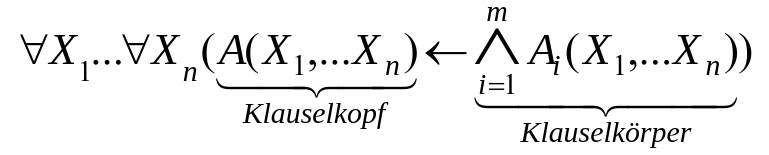
\includegraphics[width=.5\linewidth]{Assets/Logik-prolog-horn.png}

  \begin{enumerate*}
    \item Regeln (vollständige HORN-Klauseln)        $\forall X_1... \forall X_n(A(X_1,...,X_n)\leftarrow \bigwedge_{i=1}^n A_i(X_1,...,X_n))$
    \item Fakten (HORN-Klauseln mit leerem Klauselkörper)        $\forall X_1...\forall X_n(A(X_1,...,X_n)\leftarrow true)$
    \item Fragen (HORN-Klauseln mit leerem Klauselkopf)        $\forall X_1...\forall X_n(false \leftarrow \bigwedge_{i=1}^n A_i(X_1,...,X_n))$
    \item leere HORN-Klauseln (mit leeren Kopf \& leerem Körper)        $false\leftarrow true$
  \end{enumerate*}

  Effekte der Beschränkung auf HORN-Logik
  \begin{enumerate*}
    \item Über HORN-Klauseln gibt es ein korrektes und vollständiges Ableitungsverfahren. $\{K_1, ...,K_n\} \Vdash H$ , gdw. $\{K_1,...,K_n\} \vdash_{ROB} H$
    \item Die Suche nach einer Folge von Resolutionsschritten ist algorithmisierbar.
    \begin{itemize*}
      \item Das Verfahren ''Tiefensuche mit Backtrack'' sucht systematisch eine Folge, die zur leeren Klausel führt.
      \item Rekursive und/oder metalogische Prädikate stellen dabei die Vollständigkeit in Frage.
    \end{itemize*}
    \item Eine Menge von HORN-Klauseln mit nichtleeren Klauselköpfen ist stets erfüllbar; es lassen sich keine Widersprüche formulieren. $K_1 \wedge K_2...\wedge K_n \not= false$
  \end{enumerate*}

  Die systematische Erzeugung von (HORN-) Klauseln
  \begin{enumerate*}
    \item Verneinungstechnischen Normalform (VTNF): $\lnot$ steht nur vor Atomformeln $\lnot\lnot A\equiv A$
    \item Erzeugung der Pränexen Normalform (PNF): $\forall, \exists$ stehen vor dem Gesamtausdruck
    \begin{itemize*}
      \item $\forall X A(X) \rightarrow B \equiv \exists X(A(X)\rightarrow B)$
      \item $\exists X A(X) \rightarrow B \equiv \forall X(A(X)\rightarrow B)$
    \end{itemize*}
    \item Erzeugung der SKOLEM‘schen Normalform (SNF): $\exists$ wird eliminiert
    \item Erzeugung der Konjunktiven Normalform (KNF): Durch systematische Anwendung des Distributivgesetzes $A\vee (B\wedge C)\equiv (A\vee B)\wedge(A\vee C)$
    \item Erzeugung der Klauselform (KF): Jede der Elementardisjunktionen $(L_1^j \vee...\vee L_1^{j_k})$ der KNF kann man als äquivalente Implikation (Klausel) $(L_i^j \vee...\vee L_i^{j_m})\leftarrow(L_1^{j_{m+1}}\wedge ...\wedge L_1^{j_k})$ notieren, indem man alle positiven Literale $L_i^j,...,L_i^{j_m}$ disjunktiv verknüpft in den DANN-Teil (Klauselkopf) und alle negativen Literale $L_i^{j_{m+1}},...,L_i^{j_k}$ konjunktiv verknüpft in den WENN-Teil (Klauselkörper) notiert.
    \item In dem Spezialfall, dass alle Klauselköpfe dabei aus genau einem Literal bestehen, war die systematische Erzeugung von HORN-Klauseln erfolgreich; anderenfalls gelingt sie auch nicht durch andere Verfahren.
  \end{enumerate*}

  \subsubsection{Inferenz in PROLOG: Resolution nach ROBINSON}
  \note{Satz von ROBINSON}{$M'\equiv\bigwedge_{i=1}^n K_i\wedge \lnot H$ ist kontradiktorisch ($kt\ M‘$), gdw. durch wiederholte Resolutionen in endlich vielen Schritten die negierte Hypothese $\lnot H\equiv false \leftarrow H$ durch die leere Klausel $false\leftarrow true$ ersetzt werden kann.}

  Substitution
  \begin{itemize*}
    \item Eine Substitution $\nu$ einer Atomformel $A$ ist eine Abbildung der Menge der in $A$ vorkommenden Variablen $X$ in die Menge der Terme
    \item Sie kann als Menge von Paaren $[Variable,Ersetzung]$ notiert werden: $\nu=\{[x,t]: x\in X, t=\nu(x)\}$
    \item Für strukturierte Terme wird die Substitution auf deren Komponenten angewandt: $\nu(f(t_1,...,t_n)) = f(\nu(t_1),...,\nu(t_n))$
    \item Verkettungsoperator $\circ$ für Substitutionen drückt Hintereinander-anwendung aus: $\sigma\circ\nu(t)=\sigma(\nu(t))$
    \item Substitutionen, die zwei Terme syntaktisch identisch machen, heißen Unifikator: $\nu$unifiziert zwei Atomformeln $s$ und $t$, falls dessen Einsetzung $s$ und $t$ syntaktisch identisch macht.
  \end{itemize*}

  \paragraph{Unifikation}
  Zwei Atomformeln $p(t_{11},...,t_{1n})$ und $p_2(t_{21},...,t_{2n})$ sind unifizierbar, gdw.
  \begin{itemize*}
    \item sie die gleichen Prädikatensymbole aufweisen ($p_1= p_2$),
    \item sie die gleichen Stelligkeiten aufweisen ($n = m$) und
    \item die Terme $t_{1i}$ und $t_{2i}$ jeweils miteinander unifizierbar sind.
  \end{itemize*}

  Die Unifizierbarkeit zweier Terme richtet sich nach deren Sorte:
  \begin{enumerate*}
    \item Zwei Konstanten $t_1$ und $t_2$ sind unifizierbar, gdw. $t_1= t_2$
    \item Zwei strukturierte Terme $f(t_{11},...,t_{1n})$ und $f(t_{21},...,t_{2n})$ sind unifizierbar, gdw.
    \begin{itemize*}
      \item sie die gleichen Funktionssymbole aufweisen ($f_1= f_2$),
      \item sie die gleichen Stelligkeiten aufweisen ($n=m$) und
      \item die Terme $t_{1i}$ und $t_{2i}$ jeweils miteinander unifizierbar sind.
    \end{itemize*}
    \item Eine Variable $t_1$ ist mit einer Konstanten oder einem strukturierten Term $t_2$ unifizierbar. $t_1$ wird durch $t_2$ ersetzt (instanziert): $t_1:= t_2$
    \item Zwei Variablen $t_1$ und $_2$ sind unifizierbar und werden gleichgesetzt: $t_1:=t_2$ bzw. $t_2:= t_1$
  \end{enumerate*}

  \note{Allgemeinster Unifikator}{Eine Substitution heißt allgemeinster Unifikator zweier Terme $s$ und $t$ ($\nu= m.g.u.(s,t)$), gdw.
    \begin{enumerate*}
      \item die Substitution $\nu$ ein Unifikator von $s$ und $t$ ist und
      \item für jeden anderen Unifikator $\sigma$ von $s$ und $t$ eine nichtleere und nicht identische Substitution $\tau$ existiert, so dass $\sigma=\tau\circ\nu$ ist.
    \end{enumerate*}
    %graphisch betrachtet: %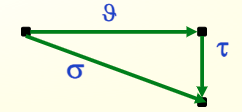
\includegraphics[width=\linewidth]{Assets/Logik_allgemeinster-unifikator.png}
  }

  Algorithmus zur Bestimmung des allgemeinsten Unifikators 2er Terme
  \begin{lstlisting}
  input: s, t
  output: Unifizierbarkeitsaussage, ggf. $\nu= m.g.u.( s , t )$
  $i:=0;\nu_i:=\varnothing;s_i:=s; t_i=t$
  Start: $s_i$ und $t_i$ identisch?
    ja $\Rightarrow$ s und t sind unifizierbar, $\nu=\nu_i=m.g.u.(s,t)$ (fertig)
    nein $\Rightarrow$ Bilde die Unterscheidungsterme $s_i^*$ und $t_i^*$
      $s_i^*$ oder $t_i^*$ Variable?
        nein $\Rightarrow$ $s$ und $t$ sind nicht unifizierbar (fertig)
        ja $\Rightarrow$ sei (o.B.d.A.) $s_i^*$ eine Variable
          $s_i^* \subseteq t_i^*$? (enthaelt $t_i^*$ die Variable $s_i^*$?)
            ja $\Rightarrow$ $s$ und $t$ sind nicht unifizierbar (fertig)
            nein $\Rightarrow$ 
              $\nu':=\{[s,t']: [s,t]\in\nu, t':=t|_{s*\rightarrow t*}\}\cup \{[s_i^*, t_i^*]\}$
              $s':=\nu'(s_i); t':=\nu'(t_i); i:=i+1;$
              $\nu_i:=\nu'; s_i:=s'; t_i:=t';$ 
              gehe zu Start
  \end{lstlisting}

  \subsection{Logische Programmierung}
  ''deskriptives'' Programmierparadigma =
  \begin{enumerate*}
    \item Problembeschreibung
    \begin{itemize*}
      \item Die Aussagenmenge $M =\{K_1,...,K_n\}$, über denen gefolgert wird, wird in Form von Fakten und Regeln im PK1 notiert.
      \item Eine mutmaßliche Folgerung (Hypothese) $H$ wird in Form einer Frage als negierte Hypothese hinzugefügt.
    \end{itemize*}
    \item (+) Programmverarbeitung
    \begin{itemize*}
      \item Auf der Suche eines Beweises für $M \Vdash H$ werden durch mustergesteuerte Prozedur-Aufrufe Resolutions-Schritte zusammengestellt.
      \item Dem ''Programmierer'' werden (begrenzte) Möglichkeiten gegeben, die systematische Suche zu beeinflussen.
    \end{itemize*}
  \end{enumerate*}

  \subsubsection{Syntax}
  BACKUS-NAUR-Form
  \begin{itemize*}
    \item PROLOG-Programm ::= Wissensbasis Hypothese
    \item Wissensbasis ::= Klausel | Klausel Wissensbasis
    \item Klausel ::= Fakt | Regel
    \item Fakt ::= Atomformel.
    \item Atomformel ::= Prädikatensymbol (Termfolge)
    \item Prädikatensymbol ::= Name
    \item Name ::= Kleinbuchstabe | Kleinbuchstabe Restname | ''Zeichenfolge'' | Sonderzeichenfolge
    \item RestName ::= Kleinbuchstabe | Ziffer | $\_$ | Kleinbuchstabe RestName | Ziffer RestName | \_ RestName
    \item ...
  \end{itemize*}

  Was muss der Programmierer tun?
  \begin{itemize*}
    \item Formulierung einer Menge von Fakten und Regeln
    \item Formulierung einer negierten Hypothese (Frage, Ziel)
  \end{itemize*}

  Was darf der Programmierer erwarten? Dass das ''Deduktionstool'' PROLOG $M \Vdash H$ zu zeigen versucht, indem systematisch die Resolutionsmethode auf $\lnot H$ und eine der Klauseln aus $M$ angewandt wird, solange bis $\lnot H\equiv false\leftarrow true$ entsteht

  \paragraph{Formulierung von Wissensbasen}
  Visual Prolog benötigt aber einen Deklarationsteil für Datentypen und Aritäten der Prädikate
  \begin{lstlisting}
  domains
    person = symbol
  predicates
    vater_von(person,person)       
    mutter_von(person,person).     
    grossvater_von(person,person)   
    geschwister(person,person)      
  clauses
    < Wissensbasis einfuegen >
    // Klauseln gleichen Kopfpraedikates gruppieren
  goal
    < Frage ohne ''?-'' einfuegen>
  \end{lstlisting}

  \paragraph{Verarbeitung Logischer Programme}
  \paragraph{Veranschaulichung ohne Unifikation}
  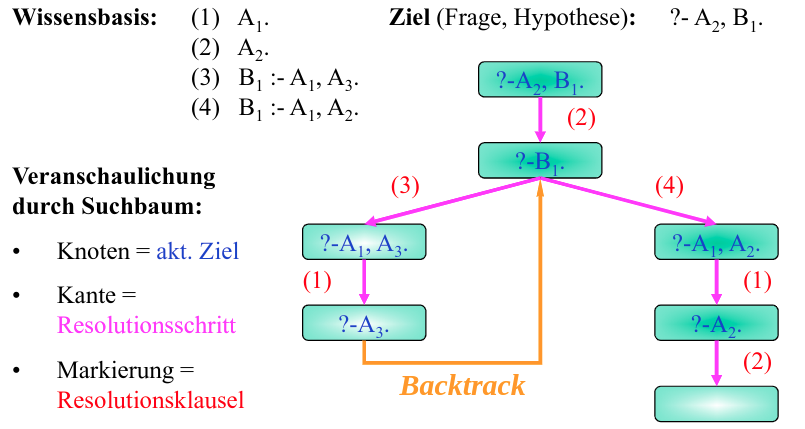
\includegraphics[width=.5\linewidth]{Assets/Logik-prolog-ohne-unifikation.png}

  Tiefensuche mit Backtrack:
  Es werden anwendbare Klauseln für das erste Teilziel gesucht. Gibt es ...
  \begin{itemize*}
    \item ... genau eine, so wird das 1. Teilziel durch deren Körper ersetzt.
    \item ... mehrere, so wird das aktuelle Ziel inklusive alternativ anwendbarer Klauseln im Backtrack-Keller abgelegt und die am weitesten oben stehende Klausel angewandt.
    \item ... keine (mehr), so wird mit dem auf dem Backtrack-Keller liegendem Ziel die Bearbeitung fortgesetzt.
  \end{itemize*}

  Dies geschieht solange, bis
  \begin{itemize*}
    \item das aktuelle Ziel leer ist oder
    \item keine Klausel (mehr) anwendbar ist und der Backtrack-Keller leer ist.
  \end{itemize*}


  \paragraph{Veranschaulichung mit Unifikation}
  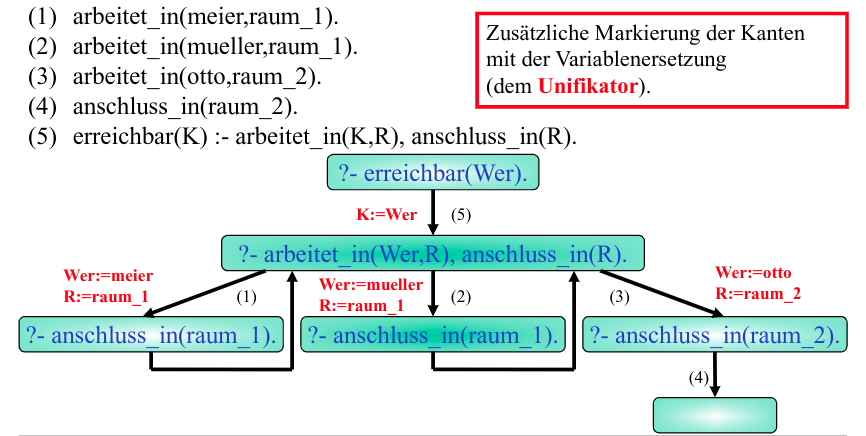
\includegraphics[width=.5\linewidth]{Assets/Logik-prolog-mit-unifikation.png}

  Zusätzliche Markierung der Kanten mit der Variablenersetzung (dem Unifikator).


  \subsubsection{PROLOG aus prozeduraler Sicht}
  \note{Deklarative Interpretation}{In einem Objektbereich $I=\{mueller, mayer, schulze, ...\}$ bildet das Prädikat $weisungsrecht(X,Y)$ $[X,Y]$ auf wahr ab, gdw.
    \begin{itemize*}
      \item das Prädikat $chef_von(X,Y)$ das Paar $[X,Y]$ auf wahr abbildet oder
      \item es ein $Z\in I$ gibt, so dass
      \begin{itemize*}
        \item das Prädikat $chef_von(X,Z)$ das Paar $[X,Z]$ auf wahr abbildet und
        \item das Prädikat $weisungsrecht(Z,Y)$ das Paar $[Z,Y]$ auf wahr abbildet.
      \end{itemize*}
    \end{itemize*}
  }

  \note{Prozedurale Interpretation}{Die Prozedur $weisungsrecht(X,Y)$ wird abgearbeitet, indem
    \begin{enumerate*}
      \item die Unterprozedur $chef_von(X,Y)$ abgearbeitet wird. Im Erfolgsfall ist die Abarbeitung beendet; anderenfalls werden
      \item die Unterprozeduren $chef_von(X,Z)$ und $weisungsrecht(Z,Y)$ abgearbeitet; indem systematisch Prozedurvarianten beider Unterprozeduren aufgerufen werden. Dies geschieht bis zum Erfolgsfall oder erfolgloser erschöpfender Suche.
    \end{enumerate*}
  }

  Prädikate zur Steuerung der Suche nach einer Folge von Resolutionsschritten!

  Das Prädikat $!/0$ ist stets wahr. In Klauselkörpern eingefügt verhindert es ein Backtrack der hinter $!/0$ stehenden Teilziele zu den vor $!/0$ stehenden Teilzielen sowie zu alternativen Klauseln des gleichen Kopfprädikats. Die Verarbeitung von $!/0$ schneidet demnach alle vor der Verarbeitung verbliebenen Lösungswege betreffenden Prozedur ab.

  \subsubsection{Listen und rekursive Problemlösungsstrategien}
  Listen
  \begin{enumerate*}
    \item $[]$ ist eine Liste.
    \item Wenn $T$ ein Term und $L$ eine Liste ist, dann ist
    \begin{enumerate*}
      \item $[T|L]$ eine Liste.
      \item $T.L$ eine Liste. (ungebräuchlich)
      \item $.(T,L)$ eine Liste. (ungebräuchlich)
      \item Das erste Element $T$ heißt Listenkopf, $L$ heißt Listenkörper oder Restliste.
    \end{enumerate*}
    \item Wenn $t_1, ... ,t_n$ Terme sind, so ist $[t_1,...,t_n]$ eine Liste.
    \item Weitere Notationsformen von Listen gibt es nicht.
  \end{enumerate*}

  \subsubsection{Rekursion}
  Eine Prozedur heißt rekursiv, wenn in mindestens einem der Klauselkörper ihrer Klauseln ein erneuter Aufruf des Kopfprädikates erfolgt.
  Ist der Selbstaufruf die letzte Atomformel des Klauselkörpers der letzten Klausel dieser Prozedur - bzw. wird er es durch vorheriges ''Abschneiden'' nachfolgender
  Klauseln mit dem Prädikat $!/0$ - , so spricht man von Rechtsrekursion ; anderenfalls von Linksrekursion.
  Eine Prozedur heißt indirekt rekursiv, wenn bei der Abarbeitung ihres Aufrufes ein erneuter Aufruf derselben Prozedur erfolgt.

\subsubsection{Unifikation 2er Listen}
  \begin{enumerate*}
    \item Zwei leere Listen sind miteinander unifizierbar.
    \item Zwei nichtleere Listen $[K_1|R_1]$ und $[K_2|R_2]$ sind miteinander unifizierbar, wenn ihre Köpfe ($K_1$ und $K_2$) und ihre Restlisten ($R_1$ und $R_2$) jeweils miteinander unifizierbar sind.
    \item Eine Liste $L$ und eine Variable $X$ sind miteinander unifizierbar, wenn die Variable selbst nicht in der Liste enthalten ist. Die Variable $X$ wird bei erfolgreicher Unifikation mit der Liste $L$ instanziert: $X:=L$.
  \end{enumerate*}

  \subsubsection{Differenzlisten}
  \begin{enumerate*}
    \item Die Differenz aus einer leeren Liste und einer (beliebigen) Liste ist die leere Liste: $[] - L = []$
    \item Die Differenz aus einer Liste $[E|R]$ und der Liste $L$, welche $E$ enthält, ist die Liste $D$,
    wenn die Differenz aus $R$ und $L$ (abzügl. $E$) die Liste $D$ ist: $[E|R]-L = D$, wenn $E\in L$ und $R-(L-[E]) = D$
    \item Die Differenz aus einer Liste $[E|R]$ und einer Liste $L$, welche $E$ nicht enthält, ist die Liste $[E|D]$, wenn die Differenz aus $R$ und $L$ die Liste $D$ ist: $[E|R] - L = [E|D]$, wenn $E\in L$ und $R-L=D$
  \end{enumerate*}

  \subsubsection{Prolog-Fallen}
  \begin{itemize*}
    \item Nicht terminierende Programme
    \item Alternierende Zielklauseln: Ein aktuelles Ziel wiederholt sich und die Suche nach einer Folge von Resolutionsschritten endet nie oder die Suche nach Resolutionsschritten endet mit einem Überlauf des Backtrack-Kellers
    \item Expandierende Zielklauseln: Das erste Teilziel wird in jeden Resolutionsschritt durch mehrere neue Teilziele ersetzt; die Suche endet mit einem Speicherüberlauf
    \item Metalogische Prädikate und konstruktive Lösungen: Das Prädikat $not/1$ hat eine Aussage als Argument und ist somit eine Aussage über eine Aussage, also metalogisch.
  \end{itemize*}

  \subsubsection{Rekursive Problemlösungsstrategien}
  \note{Botschaft 1}{Man muss ein Problem nicht in allen Ebenen überblicken, um eine Lösungsverfahren zu programmieren. Es genügt die Einsicht,
    \begin{enumerate*}
      \item wie man aus der Lösung eines einfacheren Problems die Lösung des präsenten Problems macht und
      \item wie es im Trivialfall zu lösen ist.
    \end{enumerate*}
  }

  \note{Botschaft 2}{Wann immer man Objekte mit Mustern vergleicht, z.B.
    \begin{enumerate*}
      \item eine Struktur durch ''Auflegen von Schablonen'' identifiziert,
      \item Gemeinsamkeiten mehrerer Objekte identifiziert, d.h. ''eine Schablone entwirft'' oder
      \item ''gemeinsame Beispiele für mehrere Schablonen'' sucht,
    \end{enumerate*}
    mache man sich den Unifikations-Mechanismus zu nutzen.}

  \note{Botschaft 3}{Es ist mitunter leichter (oder überhaupt erst möglich), für komplexe Probleme
    \begin{enumerate*}
      \item eine potentielle Lösung zu ''erraten'' und dazu
      \item ein Verfahren zu entwickeln, welches diese Lösung auf Korrektheit testet,
    \end{enumerate*}
    als zielgerichtet die korrekte Lösung zu entwerfen. Hierbei kann man den Backtrack-Mechanismus nutzen.}

  \note{Botschaft 4}{Heuristiken sind
    \begin{enumerate*}
      \item eine Chance, auch solche Probleme einer Lösung zuzuführen, für die man keinen (determinierten) Lösungsalgorithmus kennt und
      \item das klassische Einsatzgebiet zahlreicher KI-Tools - auch der Logischen Programmierung.
    \end{enumerate*}
  }

  \note{Botschaft  5}{
    \begin{enumerate*}
      \item Für die systematische Suche eines Pfades kann der Suchprozess einer Folge von Resolutionsschritten genutzt werden. Man muss den Suchprozess nicht selbst programmieren.
    \item Für eine heuristische Suche eines Pfades gilt Botschaft 4: Sie ist das klassische Einsatzgebiet zahlreicher KI-Tools - auch der Logischen Programmierung.
    \end{enumerate*}
  }

  \note{Botschaft 6}{
    \begin{enumerate*}
      \item ''Logeleien'' sind oft Aussagen über Belegungen von Variablen mit endlichem Wertebereich, ergänzt um eine Frage zu einem nicht explizit gegebenen Wert.
      \item Dabei handelt es sich um Grunde um eine Deduktionsaufgabe mit einer Hypothese zu einem mutmaßlichen Wert der gesuchten Variablen. Deshalb ist es oft auch mit dem ''Deduktionstool'' Prolog lösbar, denn Prolog tut im Grunde nichts anderes als ein ziel-gerichtetes ''Durchprobieren'' legitimer Deduktionsschritte im ''Generate - and - Test'' - Verfahren.
    \end{enumerate*}
  }

  \note{Botschaft 7}{Auch in der formalen Logik gibt es Deduktionsaufgaben, bei der Variablenbelegungen gesucht sind, welche eine Aussage wahr machen:
    \begin{enumerate*}
      \item Meist geschieht das durch systematische Auswertung der Aussage, wozu das Suchverfahren von Prolog genutzt werden kann.
      \item Auch hier geht es oft um gesuchte Werte für Variablen. Deshalb ist es oft auch mit dem ''Deduktionstool'' Prolog lösbar, denn Prolog tut im Grunde nichts anderes als ein ziel-gerichtetes ''Durchprobieren'' legitimer Deduktionsschritte im ''Generate - and - Test'' - Verfahren.
    \end{enumerate*}
  }

\end{multicols}
\end{document}